\subsection{Transverse Field Ising model (TFIM)}
\begin{figure}[t!]
\centering
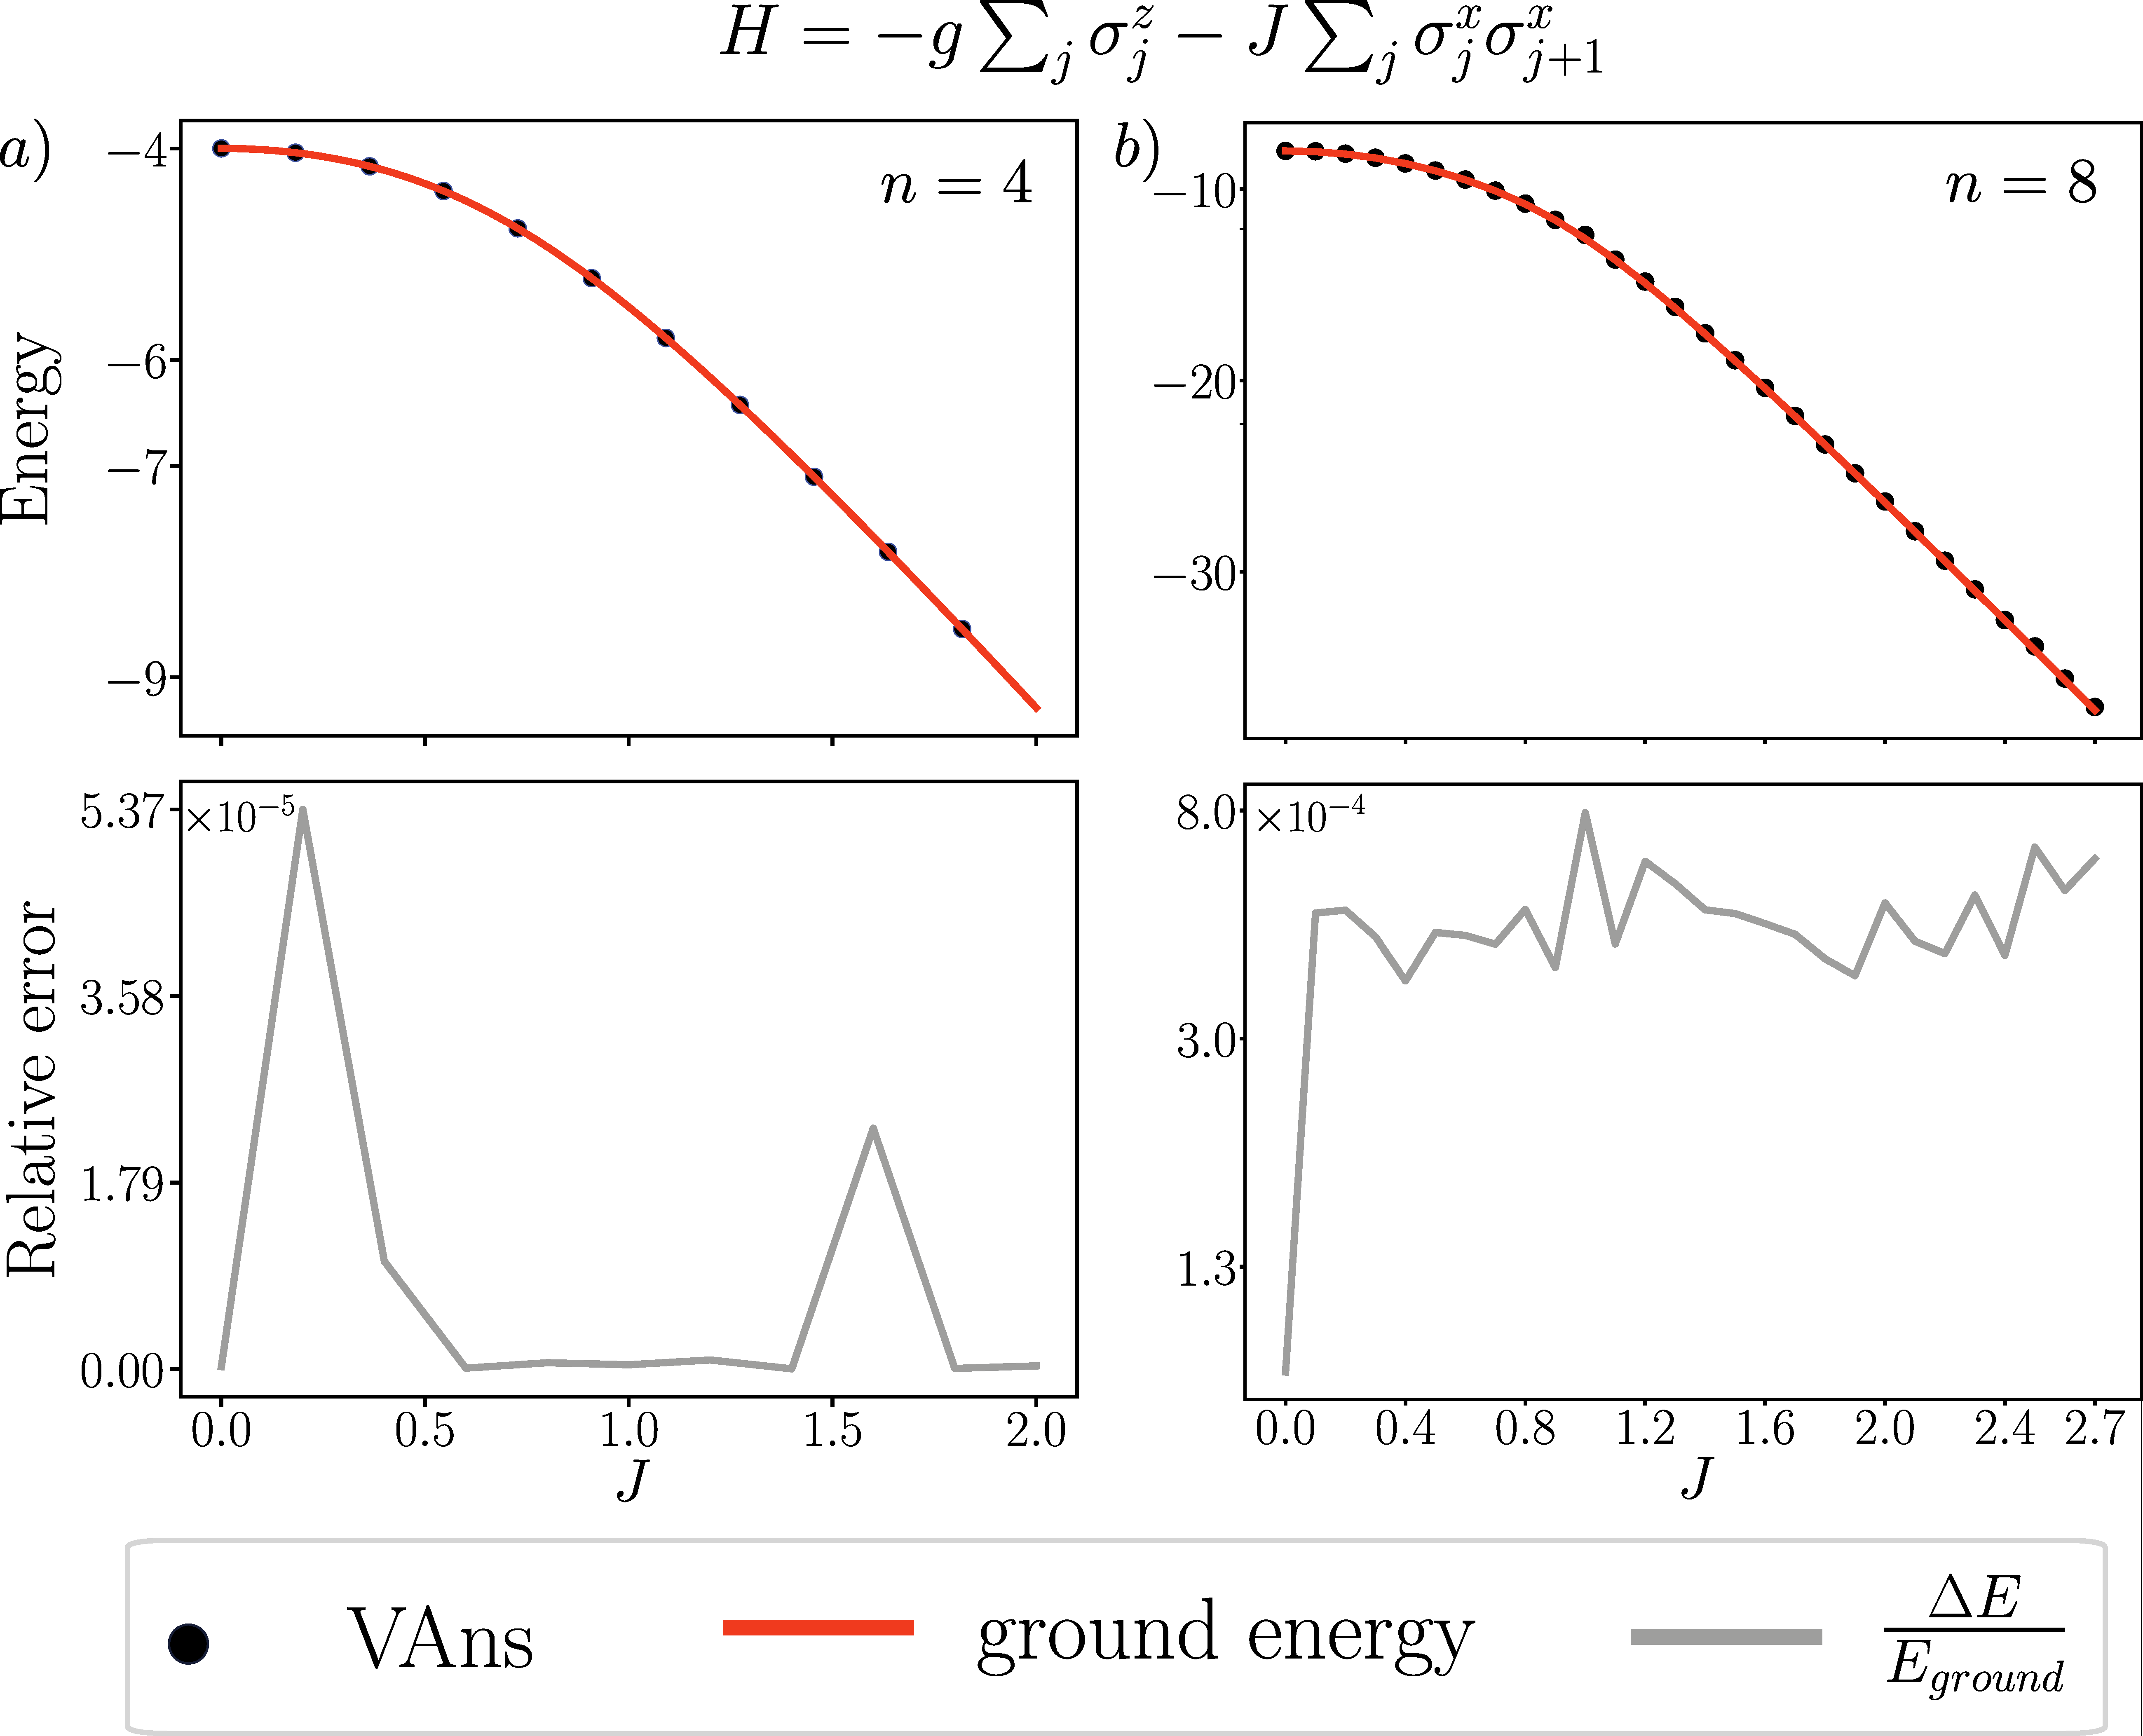
\includegraphics[width=.9\textwidth]{Figures/VANS/Fig6.pdf}
\caption{Results of using VAns to obtain the ground state of a Transverse Field Ising model: we use VAns in the VQE algorithm for the Hamiltonian in Eq.~\ref{eq:HTFIM} with \textit{(a)} $n=4$ qubits and \textit{(b)} $n=8$ qubits, field $g=1$, for different values of the interaction $J$. Top panels: solid lines indicate the exact ground state energy, and the markers are the energies obtained using VAns. Bottom panels: Relative error in the energy for the same interaction values.}
\label{fig:TFIM}
\end{figure}
\begin{figure}[t!]
\centering
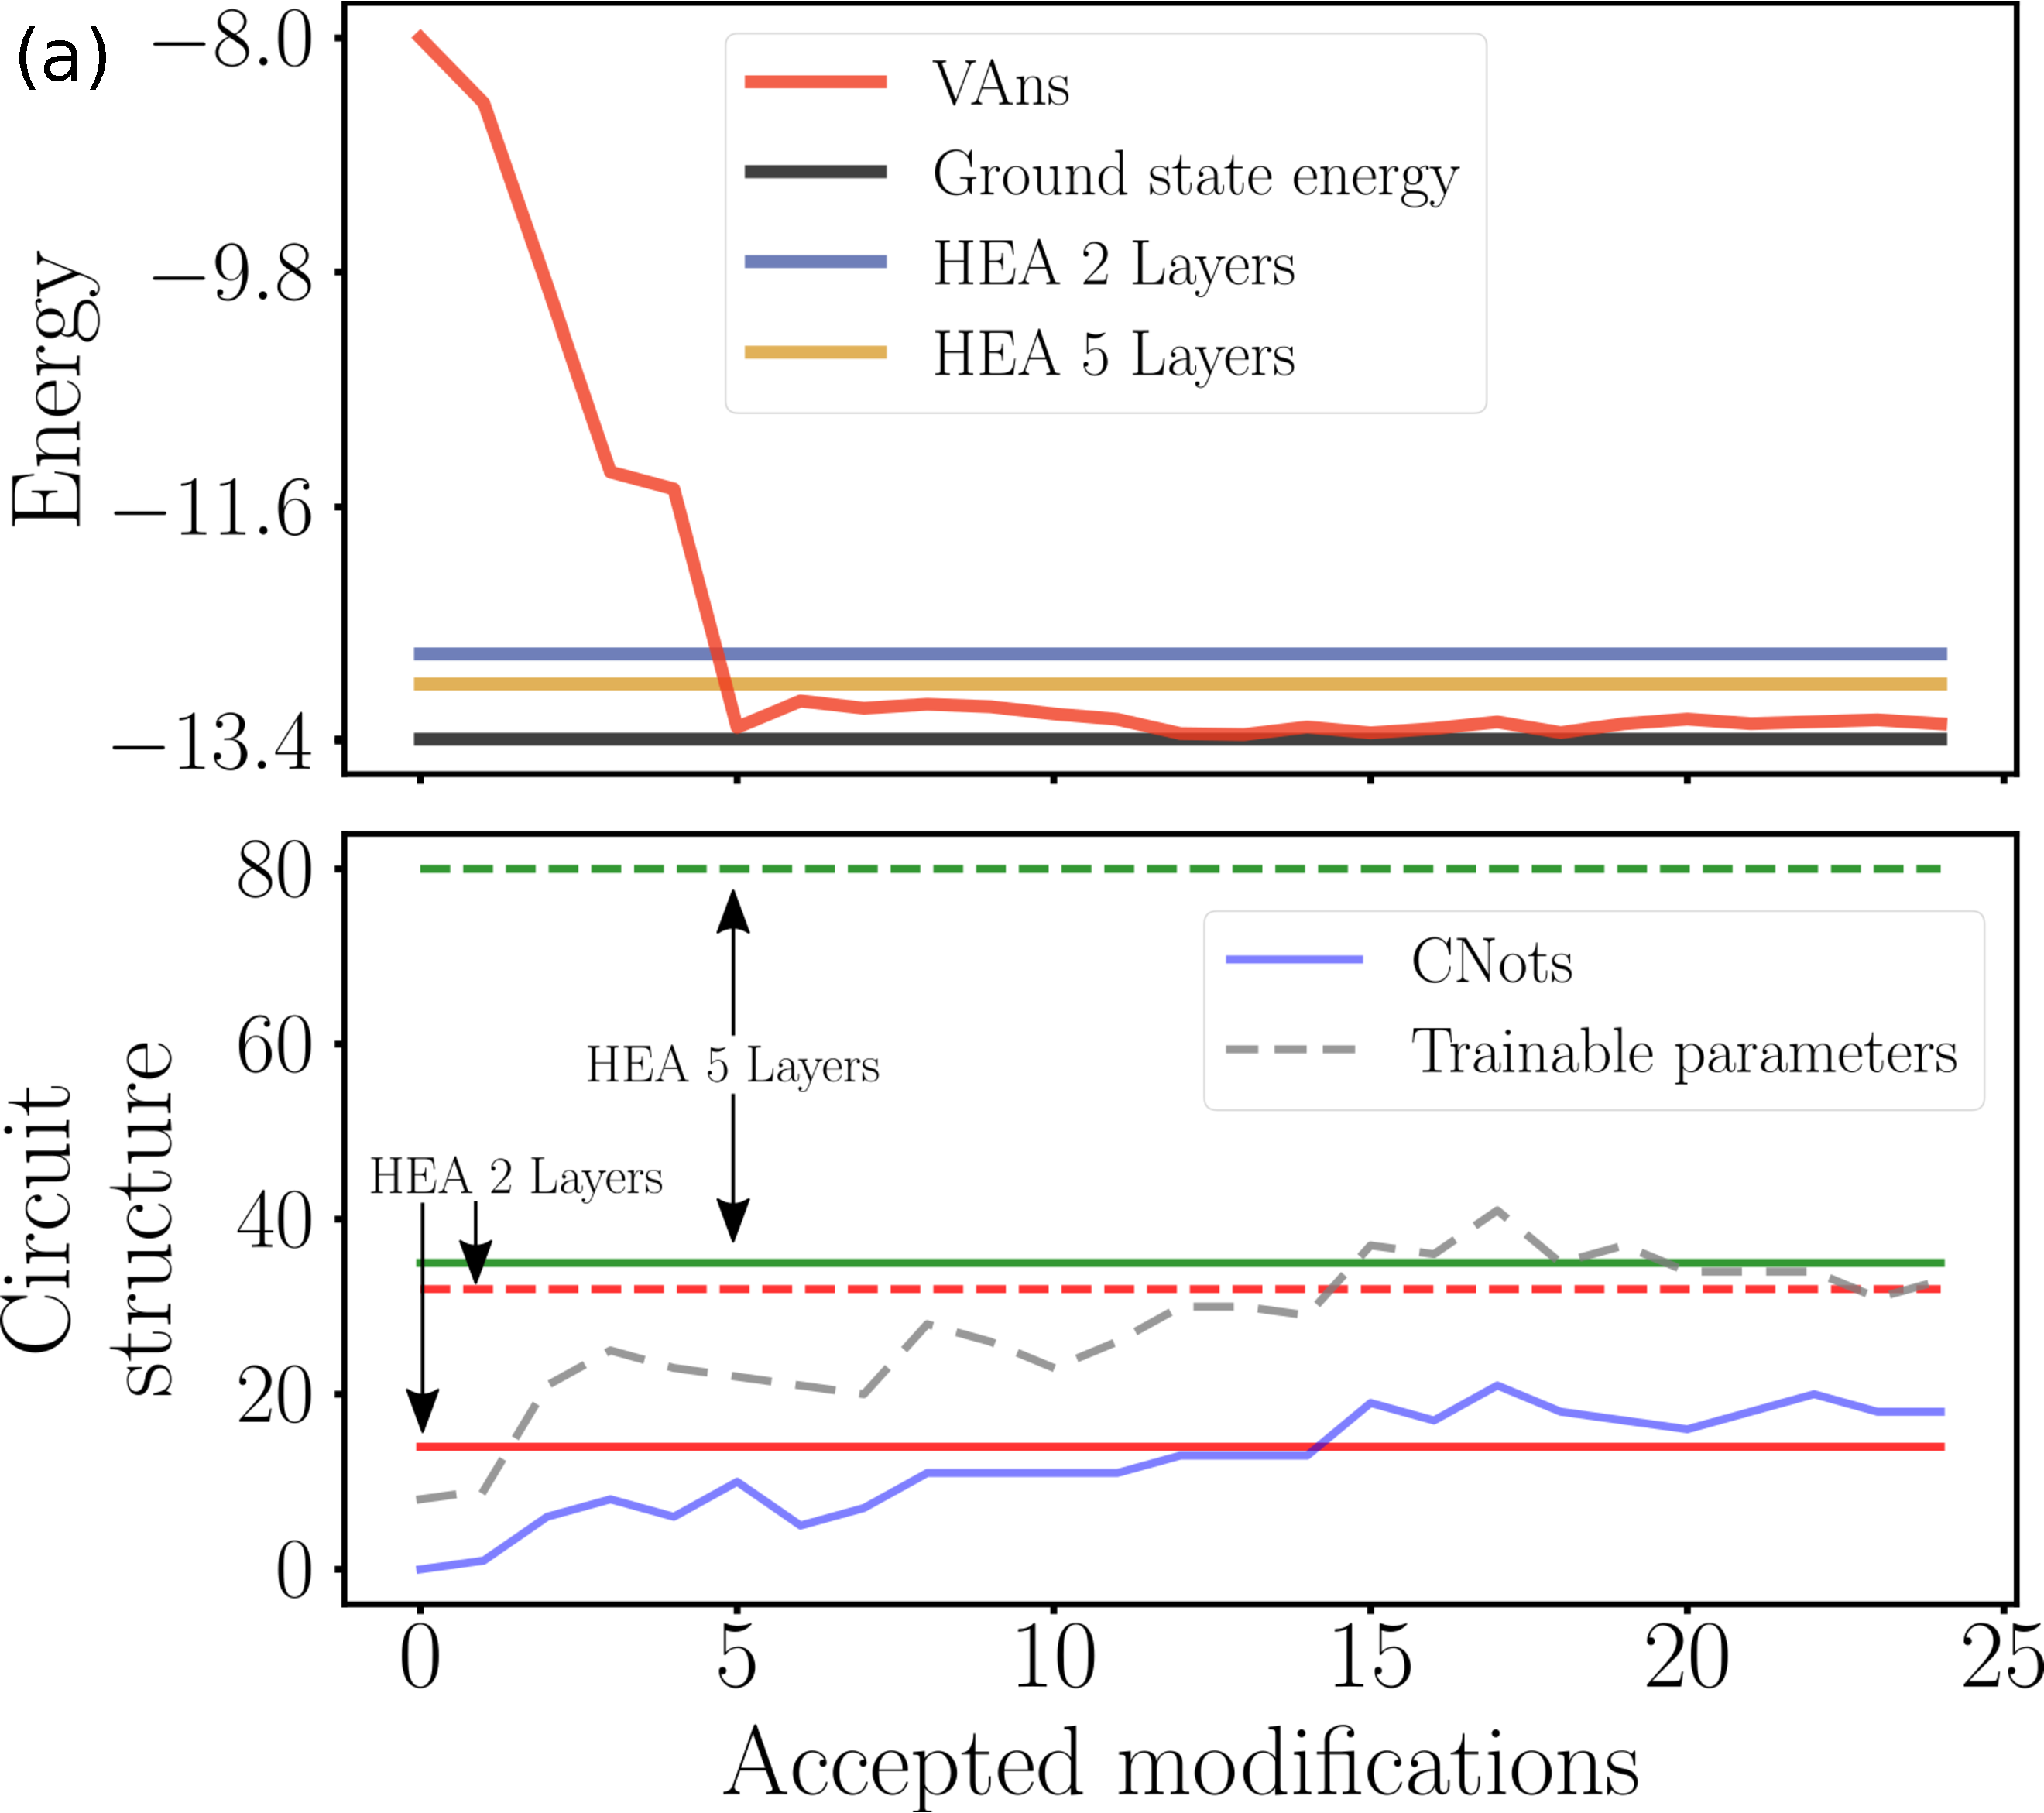
\includegraphics[width=.9\textwidth]{Figures/VANS/Fig7.pdf}
\caption{We show VAns learning process: \textit{(a)} we show an instance of running the algorithm for the Hamiltonian in Eq.~\eqref{eq:HTFIM} with $n=8$ qubits, field $g=1$, and interaction $J=1.5$. The top panel shows the cost function value and the bottom panel depicts the number of CNOTs, and the number of trainable parameters versus the number of modifications of the ansatz accepted in the VAns algorithm. Top: As the number of iterations increases, VAns minimizes the energy until one finds the ground state of the TFIM. Here we also show the best results obtained by training a fixed structure layered Hardware Efficient Ansatz (HEA) with $2$ and $5$ layers, and in both cases, VAns outperforms the HEA. Bottom: While initially the number of CNOTs and number of trainable parameters increases, the \texttt{Simplification} method in VAns prevents the circuit from constantly growing, and can even lead to shorter depth circuits that achieve better solutions. Here we also show the number of CNOTs (solid line) and parameters (dashed line) in the HEA ansatzes considered, and we see that VAns can obtain circuits with less entangling and trainable gates. }
\label{fig:learning}
\end{figure}
We now consider a cyclic TFIM chain. The Hamiltonian of the system reads
\begin{equation}\label{eq:HTFIM}
    \hat{H}=-J\sum_{j=1}^n \sigma_j^x\sigma_{j+1}^x-g\sum_{j=1}^n \sigma_j^z\,,
\end{equation}
where $\sigma_j^{x(z)}$ is the Pauli $x$ ($z$) operator acting on qubit $j$, and where $n+1\equiv 1$ to indicate periodic boundary conditions. Here, $J$ indicates the interaction strength, while $g$ is the magnitude of the transverse magnetic field. As mentioned in Section~\ref{ssec:1_nisq_vqa}, when using the VQE algorithm the goal is to optimize a parametrized quantum circuit $U(\kvec,\thv)$ to prepare the ground state of $H$ so that the cost function becomes \equ{C_{\text{VQE}}(\kvec,\thv)=\tr{\hat{H} U(\kvec,\thv)\rho U^\dagger (\kvec,\thv)},}
where one usually employs $\rho=\proj{0}$ with $\ket{0}=\ket{0}^{\otimes n}$.% Note that we here employ $E$ as the cost function label to keep with usual notation convention: in VQE applications the cost-function reduces to system's energy.

\begin{figure}[h]
\centering
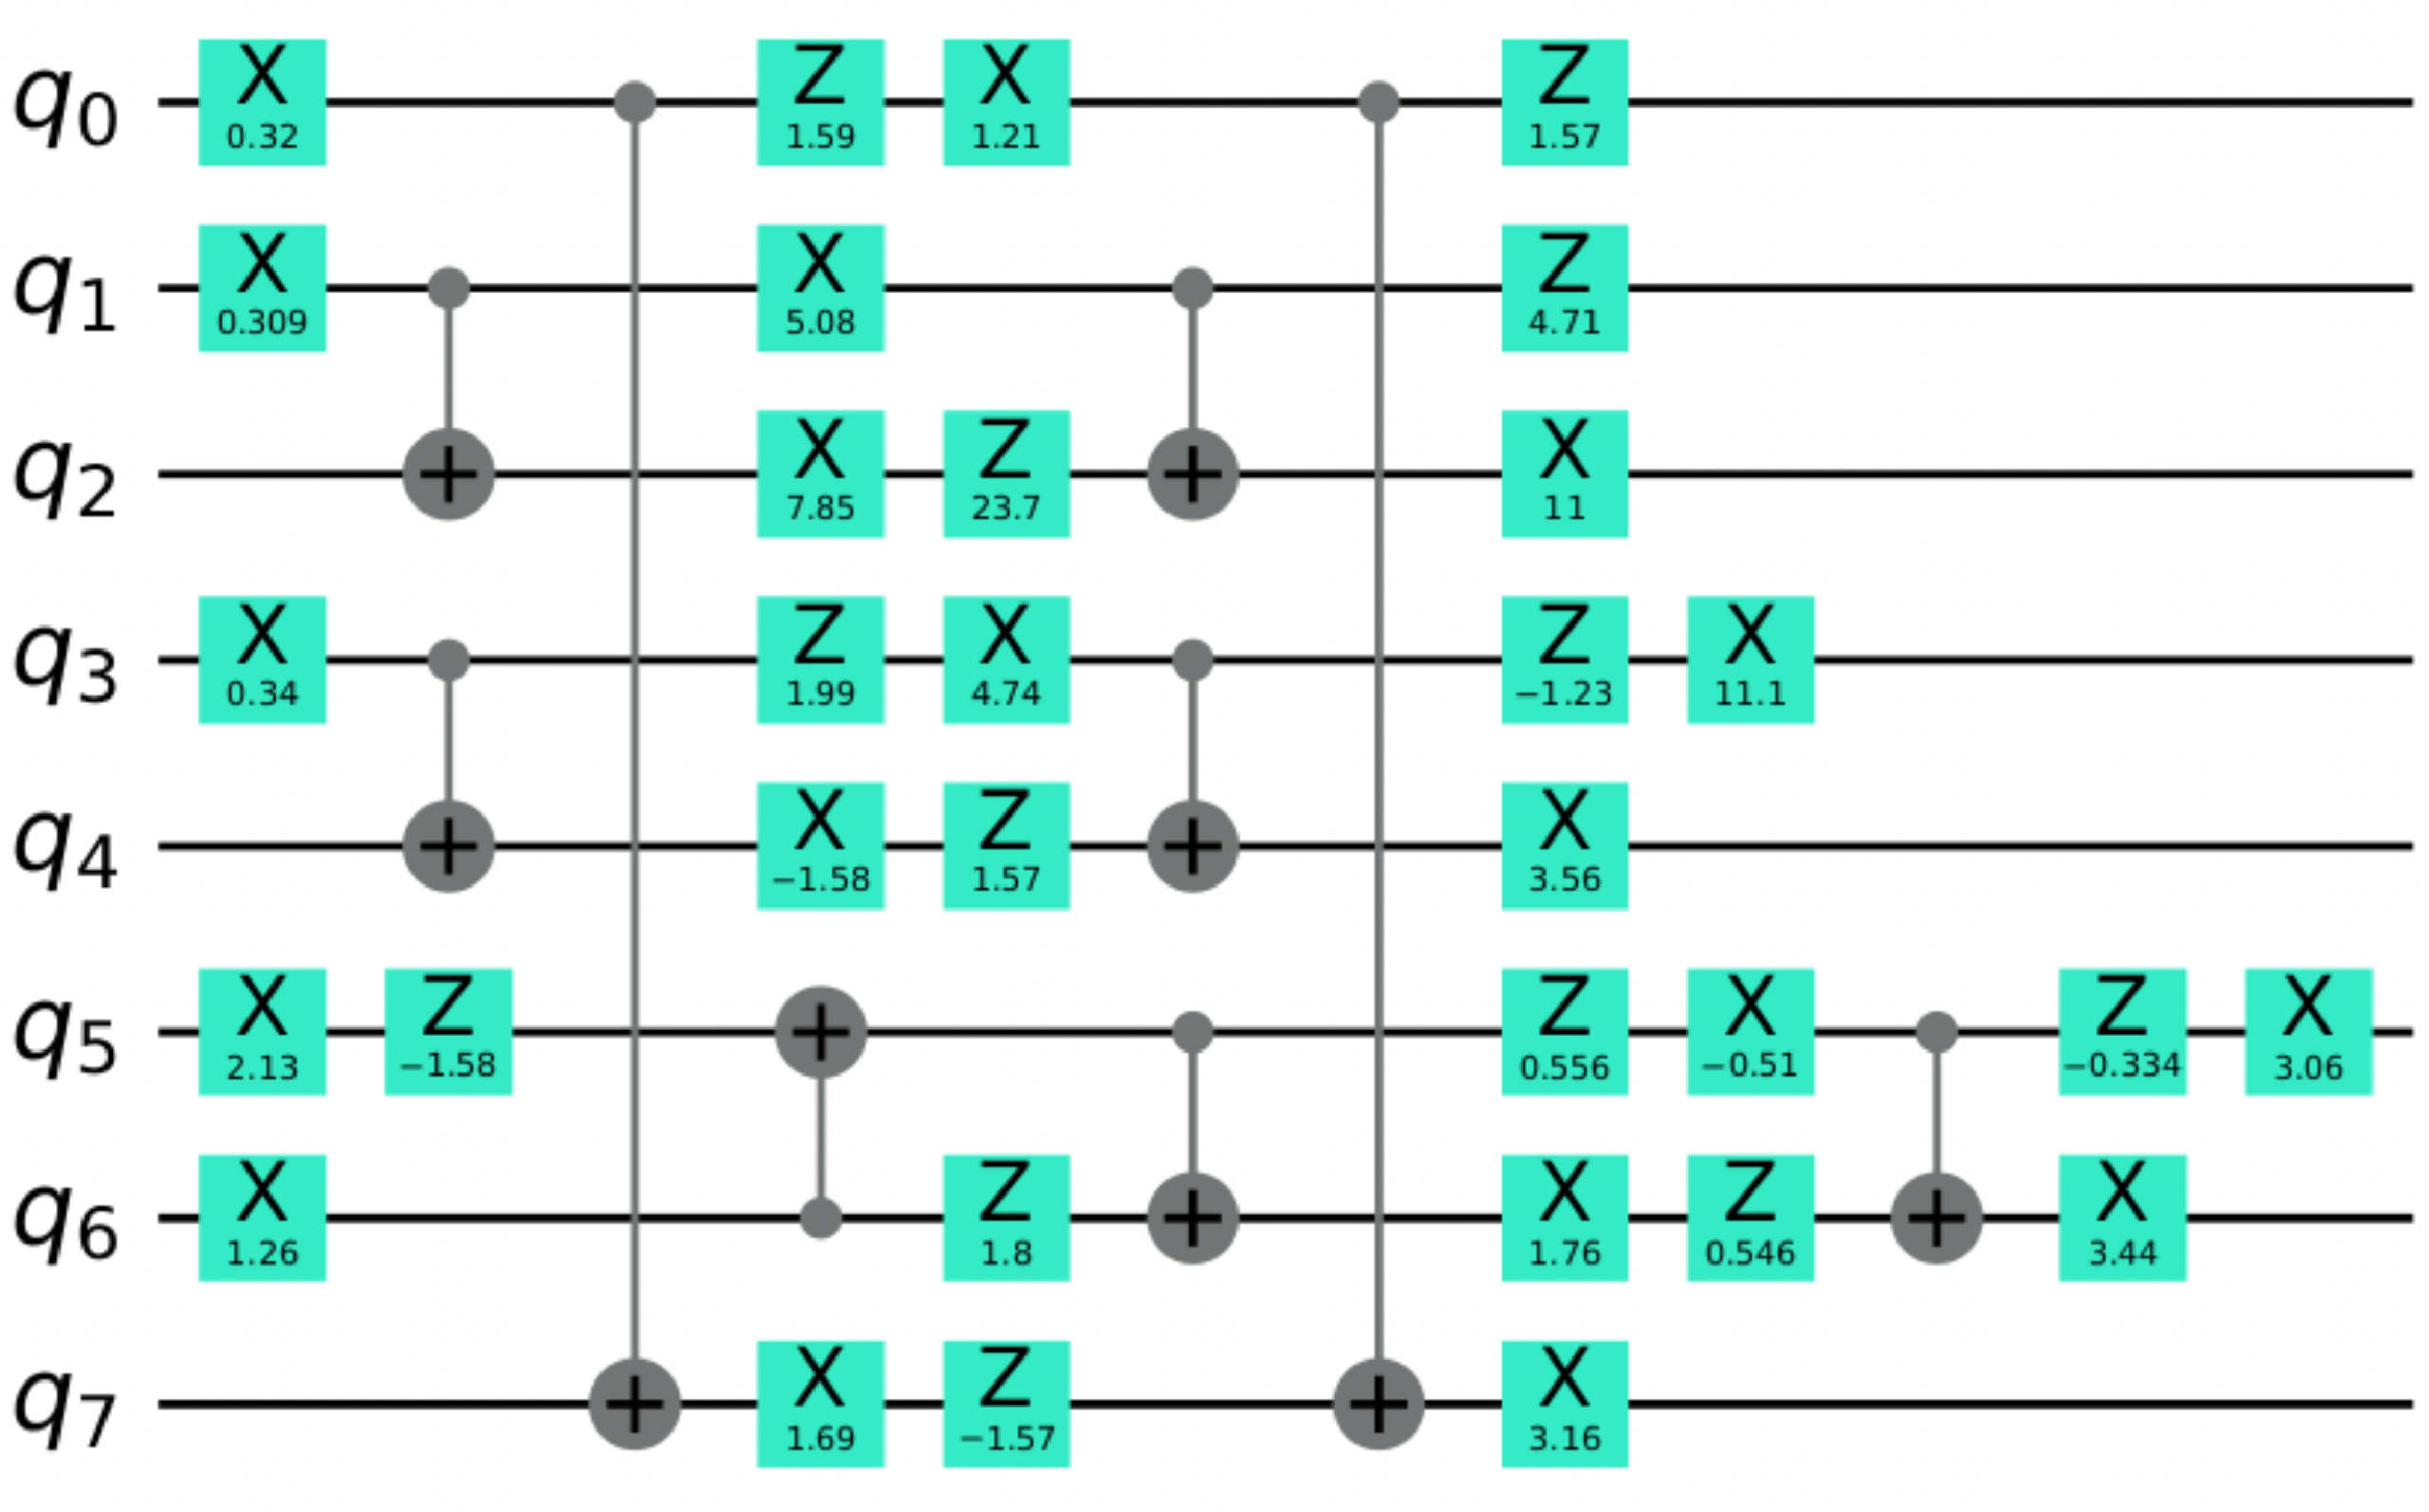
\includegraphics[width=.9\textwidth]{Figures/VANS/circTFIM.pdf}
\caption{We show a low-depth, ground-state preparing circuits found by VAns during the learning process; here $Z$ ($X$) indicates a rotation about the $z$ ($x$) axis, about the corresponding value appearing below.}
\label{fig:circui}
\end{figure}

In Fig.~\ref{fig:TFIM} we show results obtained from employing VAns to find the ground state of a TFIM model of Eq.~\eqref{eq:HTFIM} with $n=4$ qubits (a) and with $n=8$ qubits (b), field $g=1$, and different interactions values. To quantify the performance of the algorithm, we  additionally show the relative error $\left|\Delta E/E_0\right|$, where $E_0$ is the exact ground state energy $E_0$, $\Delta E=E_{\text{VAns}}-E_0$, and $E_{\text{VAns}}$ the best energy obtained through VAns. For $4$ qubits, we see from Fig.~\ref{fig:TFIM} that the relative error is always smaller than $6\times 10^{-5}$, showing the that ground-state energy was obtained for all coupling values $J$. Then, for $n=8$ qubits, VAns obtains the ground state of the TFIM with relative error smaller than $8\times 10^{-4}$.

To gain some insight into the learning process, in Fig.~\ref{fig:learning} we show the cost function value, number of CNOTs, and the number of trainable parameters in the circuit discovered by VAns as different modifications of the ansatz are accepted to minimize the cost in an $n=8$ TFIM VQE implementation. Specifically, in Fig.~\ref{fig:learning}(top) we see that as VAns explores the architecture hyperspace, the cost function value continually decreases until one can determine the ground state of the TFIM. Fig.~\ref{fig:learning}(bottom) shows that initially VAns increases the number of trainable parameters and CNOTs in the circuit via the \texttt{Insertion} step. However, as the circuit size increases, the action of the \texttt{Simplification} module becomes more relevant as we see that the number of trainable parameters and CNOTs can decrease throughout the computation. Moreover, here we additionally see that reducing the number of CNOTs and trainable parameters can lead to improvements in the cost function value. The latter indicates that VAns can indeed lead to short depth ansatzes which can efficiently solve the task at hand, even without the presence of noise.

Finally, in Fig.~\ref{fig:circui} we also compare the performance of VAns with that of 2-HEA and 5-HEA. We specifically compare against those two fixed structure ansatzes as the first (latter) has a number of trainable parameters (CNOTs) comparable to those obtained in the VAns circuit. In all cases, we see that VAns can produce better results than those obtained with the Hardware Efficient Ansatz.


\subsection{$XXZ$ Heisenberg Model}
\begin{figure}[t!]
\centering
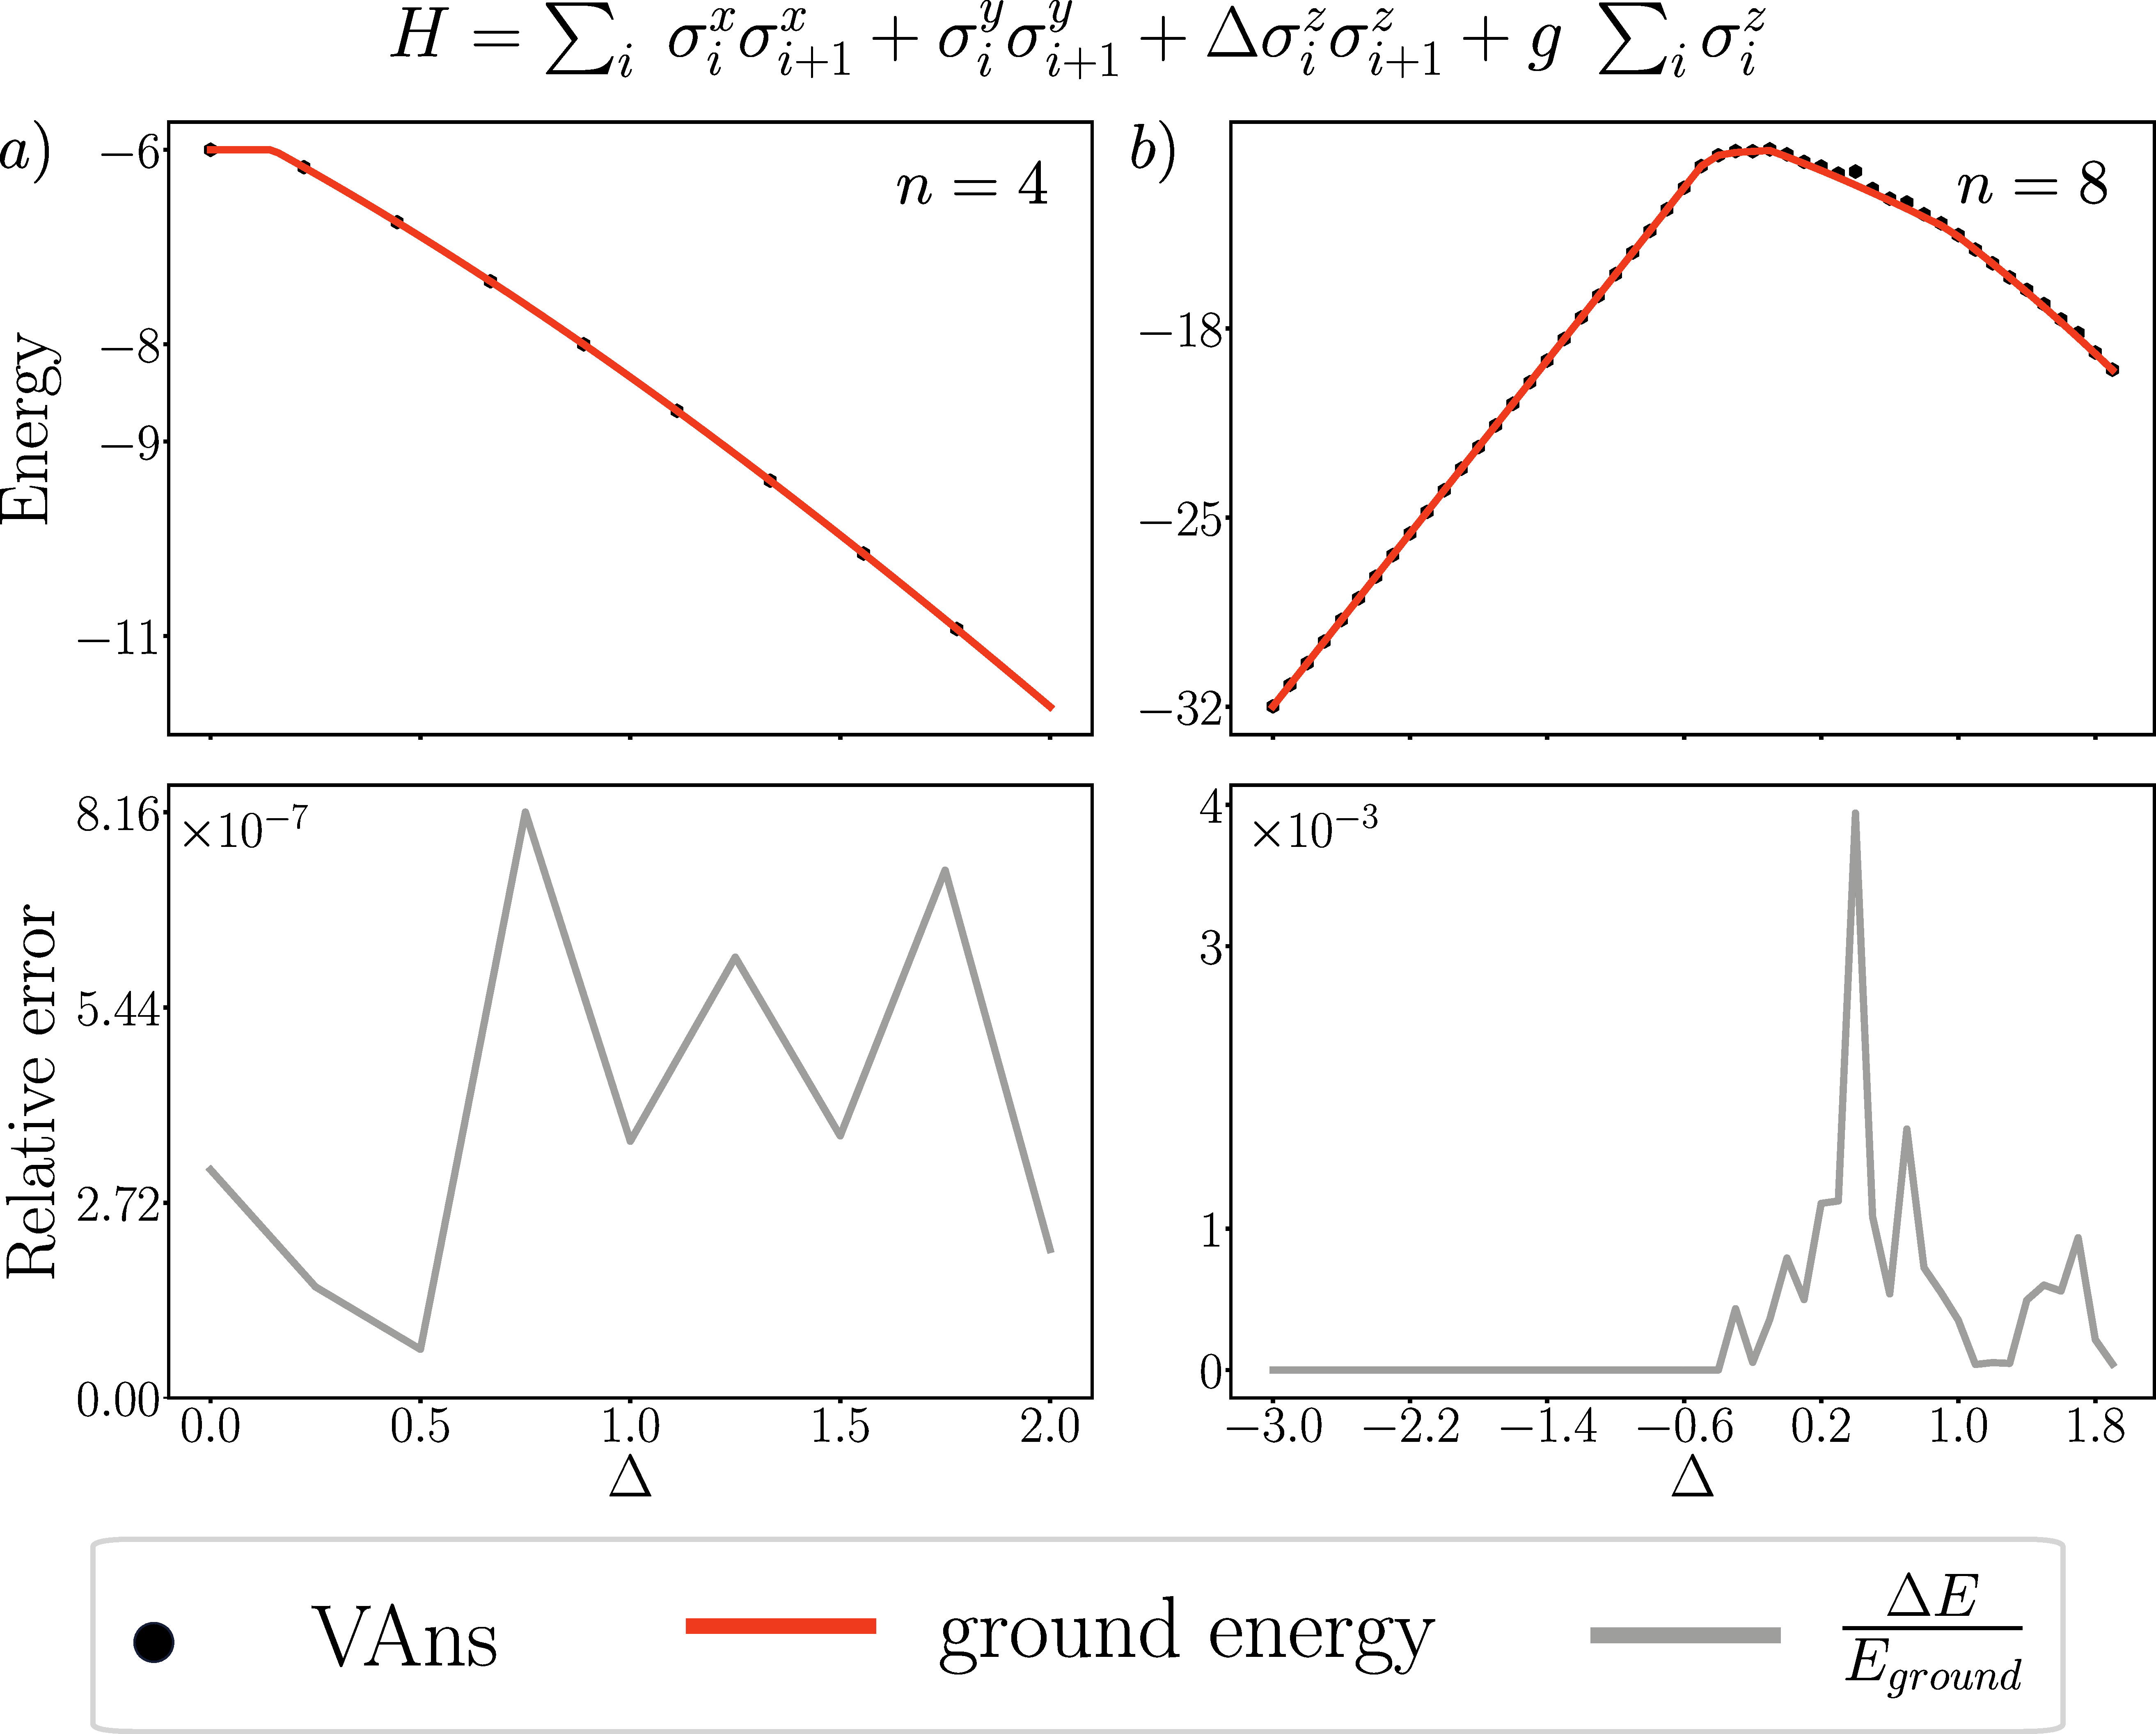
\includegraphics[width=.9\textwidth]{Figures/VANS/Fig8.pdf}
\caption{We show results of using VAns to obtain the ground state of a Heisenberg $XXZ$ model. Here, we consider the VQE algorithm for the Hamiltonian in Eq.~\ref{eq:HXXZ} with \textit{(a)} $n=4$ and \textit{(b)} $n=8$ qubits, field $g=1$, and indicated anisotropies $\Delta$. Top panels: The solid line indicates the exact ground state energy, and the markers are the energies obtained using VAns. Bottom panels: Relative error in the energy for the same anisotropy values.}
\label{fig:XXZ}
\end{figure}
Here we use VAns in a VQE implementation to obtain the ground state of a periodic $XXZ$ Heisenberg spin chain in a transverse field. The Hamiltonian of the system is
\begin{equation}\label{eq:HXXZ}
    H=\sum_{j=1}^n \sigma_j^x\sigma_{j+1}^x+\sigma_j^y\sigma_{j+1}^y+\Delta \sigma_j^z\sigma_{j+1}^z+g\sum_{j=1}^n \sigma_j^z\,,
\end{equation}
where again $\sigma_j^{\mu}$ are the Pauli operators (with $\mu=x,y,z$) acting on qubit $j$, $n+1\equiv 1$ to indicate periodic boundary conditions, and where $\Delta$ is the anisotropy. We recall that $H$ commutes with the total spin component $S_z=\sum_j \sigma^z_i$, meaning that its eigenvectors have definite magnetization $M_Z$ along $z$~\cite{cerezo2017factorization}.

In Fig.~\ref{fig:XXZ} we show numerical results for finding the ground state of~\eqref{eq:HXXZ} with $n=4$ and $n=8$ qubits, field $g=1$, and for different anisotropy values. For $4$ qubits, we see that VAns can obtain the ground-state energy with relative errors which are always smaller than $9\times 10^{-7}$. In the $n=8$ qubits case, the relative error is of the order $10^{-3}$, with error increasing in the region $0<\Delta<1$; in such case, as we discuss next, the algorithm finds the first-excited energy state.

We remark that a similar phenomenon is observed in~\cite{cervera2020meta}, where errors in preparing the ground state of the $XXZ$ chain increase in the same region. The reason behind this phenomenon is that the optimizer can get stuck in a local minimum where it prepares excited states instead of the ground state. Moreover, it can be verified that while the ground state and the three first exited states all belong to the same magnetization sub-space of state with magnetization $M_Z=0$, they have in fact different local symmetries and structure. Several of the low-lying excited states have a N\'eel-type structure of spins with non-zero local magnetization along $z$ of the form $|\uparrow\downarrow\uparrow\downarrow\cdots\rangle$. On the other hand, the state that becomes the ground-state for $\Delta>1$ is a state where all spins have zero local magnetization along $z$, meaning that the local states are in the $xy$ plane of the Bloch sphere. Since there is a larger number of excited states with a N\'eel-type structure (and with different translation symmetry) variational algorithms tend to prepare such states when minimizing the energy. Moreover, since mapping a state  with non-zero local magnetization along $z$ to a state with zero local magnetization requires a transformation acting on all qubits, any algorithm performing local updates will have a difficult time finding such mapping.



\afterpage{\clearpage}

%
\subsection{Molecular Hamiltonians}\label{ssec:molecular_ham_vans}
We will now focus on quantum chemistry problems, which consist in preparing the ground-state of a molecular hamiltonians. We will first outline how such systems can be modelled under the NISQ framework, and present our VQE-results afterwards. While our introduction to quantum chemistry suffices for the purposes of presenting the problem we benchmark VAns with, the curious reader can find more information on quantum chemistry in Refs.~\cite{RevModPhys.92.015003, mcclean2019openfermion,mcardle2020quantum}.

The molecular Hamiltonian, under the Born-Oppenheimer approximation, can be written both the phase-space and in the (fermionic) Fock space as per
\begin{align}\label{eq:Hferm}
H &= \frac{1}{2} \sum_{i\neq j} \frac{Z_i Z_j}{|\bm{R}_i -\bm{R}_j|} - \frac{1}{2} \sum_i \nabla^2_{r_i} -  \sum_{i,j} \frac{Z_j}{|\bm{R}_j - r_i|} + \sum_{i<j} \frac{1}{|r_i - r_j|}, \\
&= h_{nuc} + \sum_{pq} h_{pq}(\mathbf{R}) a_p^\dagger a_q  + \frac{1}{2} \sum_{pqrs} h_{pqrs}(\mathbf{R}) a_p^\dagger a_q^\dagger a_r a_s,
\end{align}
where we have used atomic units, and where $Z_i$ represents the nuclear charge of $i^{\text{th}}$ nuceli whose position is $\bm{R}_i$. Moreover, $a$ and $a^\dagger$ stand for the fermionic anhilation and creation operators obeying the anticommutation relations $\llaves{a_i,a^\dagger_j} = \delta_{ij}$, and we have also included the \textit{one and two-electron integrals}, which relate the phase-space representation of the Hamiltonian to the Fock-space one. To this end, we use single-electron wave-functions (known as \textit{electron spin-orbitals}, or \textit{atomic orbitals}) $\psi(\sigma)$ --- generally obtained via a Hartree-Fock approach, to be discussed shortly --- with $\sigma = (\bm{r}_i, s_i)$ representing electron's position and spin respectively, whose expression is given by
\begin{align}h_{pq}(\bm{R}) &= - \int d\sigma \phi^*_p(\sigma) \Big(\frac{\nabla^2_{\bm{r}}}{2} + \sum_i \frac{Z_i}{|\bm{R}_i - \bm{r}|} \Big) \phi_q(\sigma) \\
h_{pqrs}(\bm{R}) &= \int d\sigma_1 d\sigma_2 \frac{\phi^*_p(\sigma_1)\phi^*_q(\sigma_2)\phi_p(\sigma_1)\phi_q(\sigma_2)}{|\bm{r}_1 - \bm{r}_2|}.
\end{align}
We remark that electronic integrals depend on the geometry of the molecule under consideration, as given by the position of all nuclei $\bm{R} = \llaves{\bm{R}_j}$. Computing such integrals is a non-trivial task, and we here rely on specific libraries to do so~\cite{mcclean2019openfermion}.

From here, a basis-set of states known as \textit{molecular orbitals} is used to describe the molecule's ground-state, and many methods have been developed in the past decades to classically tackle this problem~\cite{RevModPhys.92.015003}.

The fermionic state is generally given by a superposition of Slatter determinants, generated by such basis-set (since the global state should be antisymmetric under permutations). If we aimed to obtain the exact ground state of the molecule, then we could variationally minimize its energy, and this constitutes the Full Configuration Interaction (FCI) approach; we note however that the number of determinants buildable from a given basis-set is exponentially large, and this approach is not practical --- although we have used it as a reference in our numerics ---.

On the contrary, the Hartree-Fock (HF) method keeps a single determinant, where the molecular orbitals are obtained as lineal combinations of atomic orbitals; the combination coefficients are optimized by following a mean-field approach where each electron is assumed to suffer from an effective potential generated by the remaining ones, and the state $\ket{HF}$ is thereby obtained.

However, since the HF approach treats the electrons independently, it does not capture correlation effects generally present in molecule's ground-state. To this end, an iterative approach can be considered, which applies \textit{excitation} operators to the $\ket{HF}$, in order to bring it closer to the true molecular ground-state. Each excitation swaps an electron from one molecular orbital to another, and if all excitation operators $T_n$ were to be considered, then any state could be reachable within this approach, \textit{i.e.} we get FCI.

In order to remain in the scope of classically-tractable solutions, only one and two excitation operators are often considered. To this end, the Unitary Coupled Cluster with Single and Double excitations (UCCSD) ansatz reads $\ket{\psi_{UCC}} = e^{T-T^\dagger}\ket{HF}$ with
$T = \sum_{i=1}^2 T_i$, and \equ{T_1 = \sum_{i,\alpha} t_{i,\alpha}a_i^\dagger a_\alpha, \spacee T_2 = \sum_{ij, \alpha \beta} t_{ij,\alpha \beta} a^\dagger_i a^\dagger_j a_\alpha a_\beta.}
From here, we variationally minimize the energy associated to $\ket{\psi_{UCC}}$, by modifying the coefficients $t_{i,\alpha}$ and $t_{ij,\alpha\beta}$.

As discussed in Sec.~\ref{ssec:1_nisq_vans_bp}, to implement Eq.~\ref{eq:Hferm} in a digital quantum computer one needs to map the fermionic operators into qubits operators (usually through a Jordan Wigner or Bravyi-Kitaev transformation). Here we employed the OpenFermion package~\cite{mcclean2019openfermion} to map Eq.~\ref{eq:Hferm} into a Hamiltonian expressed as a linear combination of $n$-qubit Pauli strings of the form
\begin{equation}\label{eq:HfermJW}
    H=\sum_{\vec{z}} c_{\vec{z}} P_{\vec{z}}\,,
\end{equation}
with $P_{\vec{z}}\in\{\id,\sigma^x,\sigma^y,\sigma^z\}^{\otimes n}$, $c_{\vec{z}}$ real coefficients, and $\vec{z}\in\{0,x,y,z\}^{\otimes n}$. As stressed above, note that the coefficients $c_{\vec{z}}$ generally depend on the electronic integrals, which in turn depend on the geometry of the molecule under consideration.

In all cases, the basis set used to approximate atomic orbitals was the \textit{STO-3g} one, a neutral molecule was considered, and the Jordan-Wigner transformation was used. While for the $H_2$ the number of qubits required is four ($n=4$), this number is doubled for the $H_4$ chain ($n=8$). Here, we note that the $H_4$ chain that we consider might not be found in equilibrium conditions (\textit{e.g.} the geometry that we consider may not be stable). This consists on an equally-separated array of Hydrogen atoms, by a distance that we deem \textit{bond-length}, and in our numerics we vary such distance in order to reconstruct the energy curve.

Thus, in Fig.~\ref{fig:H4} we show the results obtained for finding the ground-state energy of the Hydrogen molecule (left) and $H4$ chain (right), at different bond lengths. As stressed above, equal bond distance were considered for the $H4$ chain. Noticeably, the dictionary of gates $\mathcal{D}$ chosen here is not a \textit{chemical-inspired} one (e.g., it does not contain single and double excitation operators nor its hardware-efficient implementations), yet VAns is able to find ground-state preparing circuits within \textit{chemical accuracy}, a term which stands for the ultimate accuracy experimentally reachable in these systems~\cite{mcardle2020quantum}. Moreover, as shown in the bottom panels, VAns usually requires less than $15$ iterations until reaching convergence, showing that the algorithm quickly finds a way through the architecture hyperspace towards a solution.

\begin{figure}[b!]
\centering
  \begin{subfigure}[b]{.49\textwidth}
      \centering
      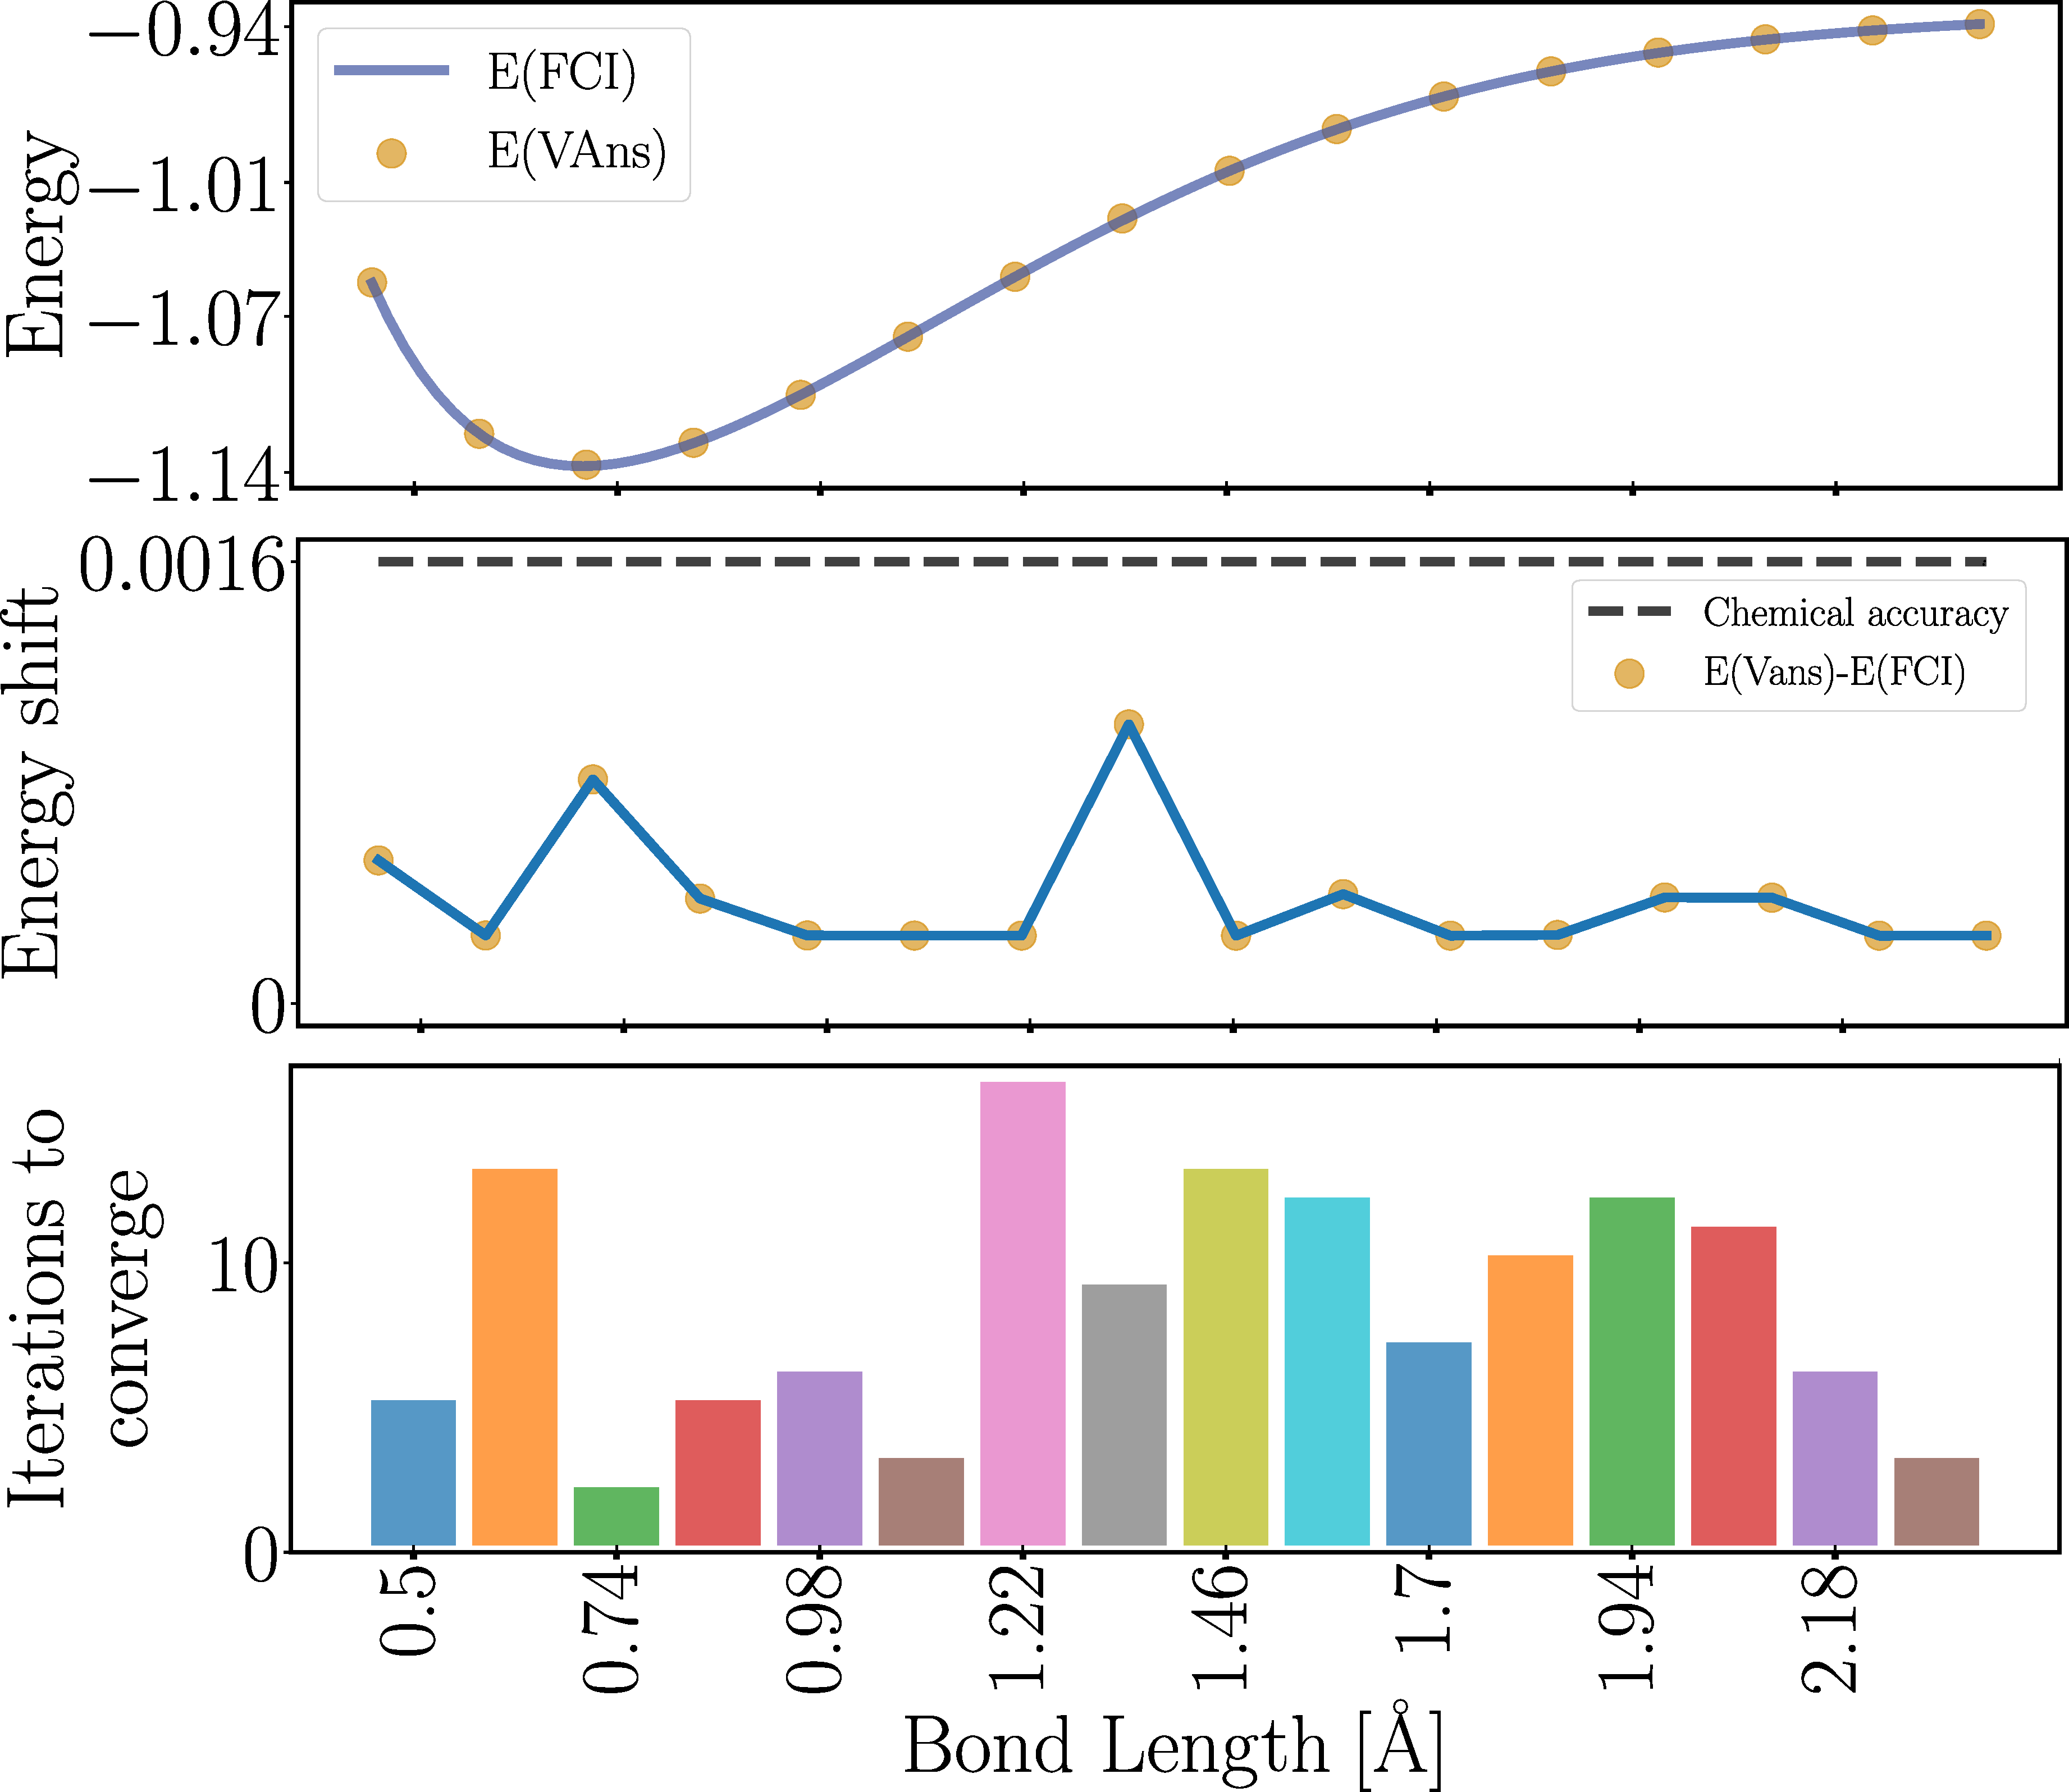
\includegraphics[width=1.\textwidth]{Figures/VANS/Fig9.pdf}
      \caption{}
      \label{fig:h22}
  \end{subfigure}
  \hfill
  \begin{subfigure}[b]{.49\textwidth}
      \centering
      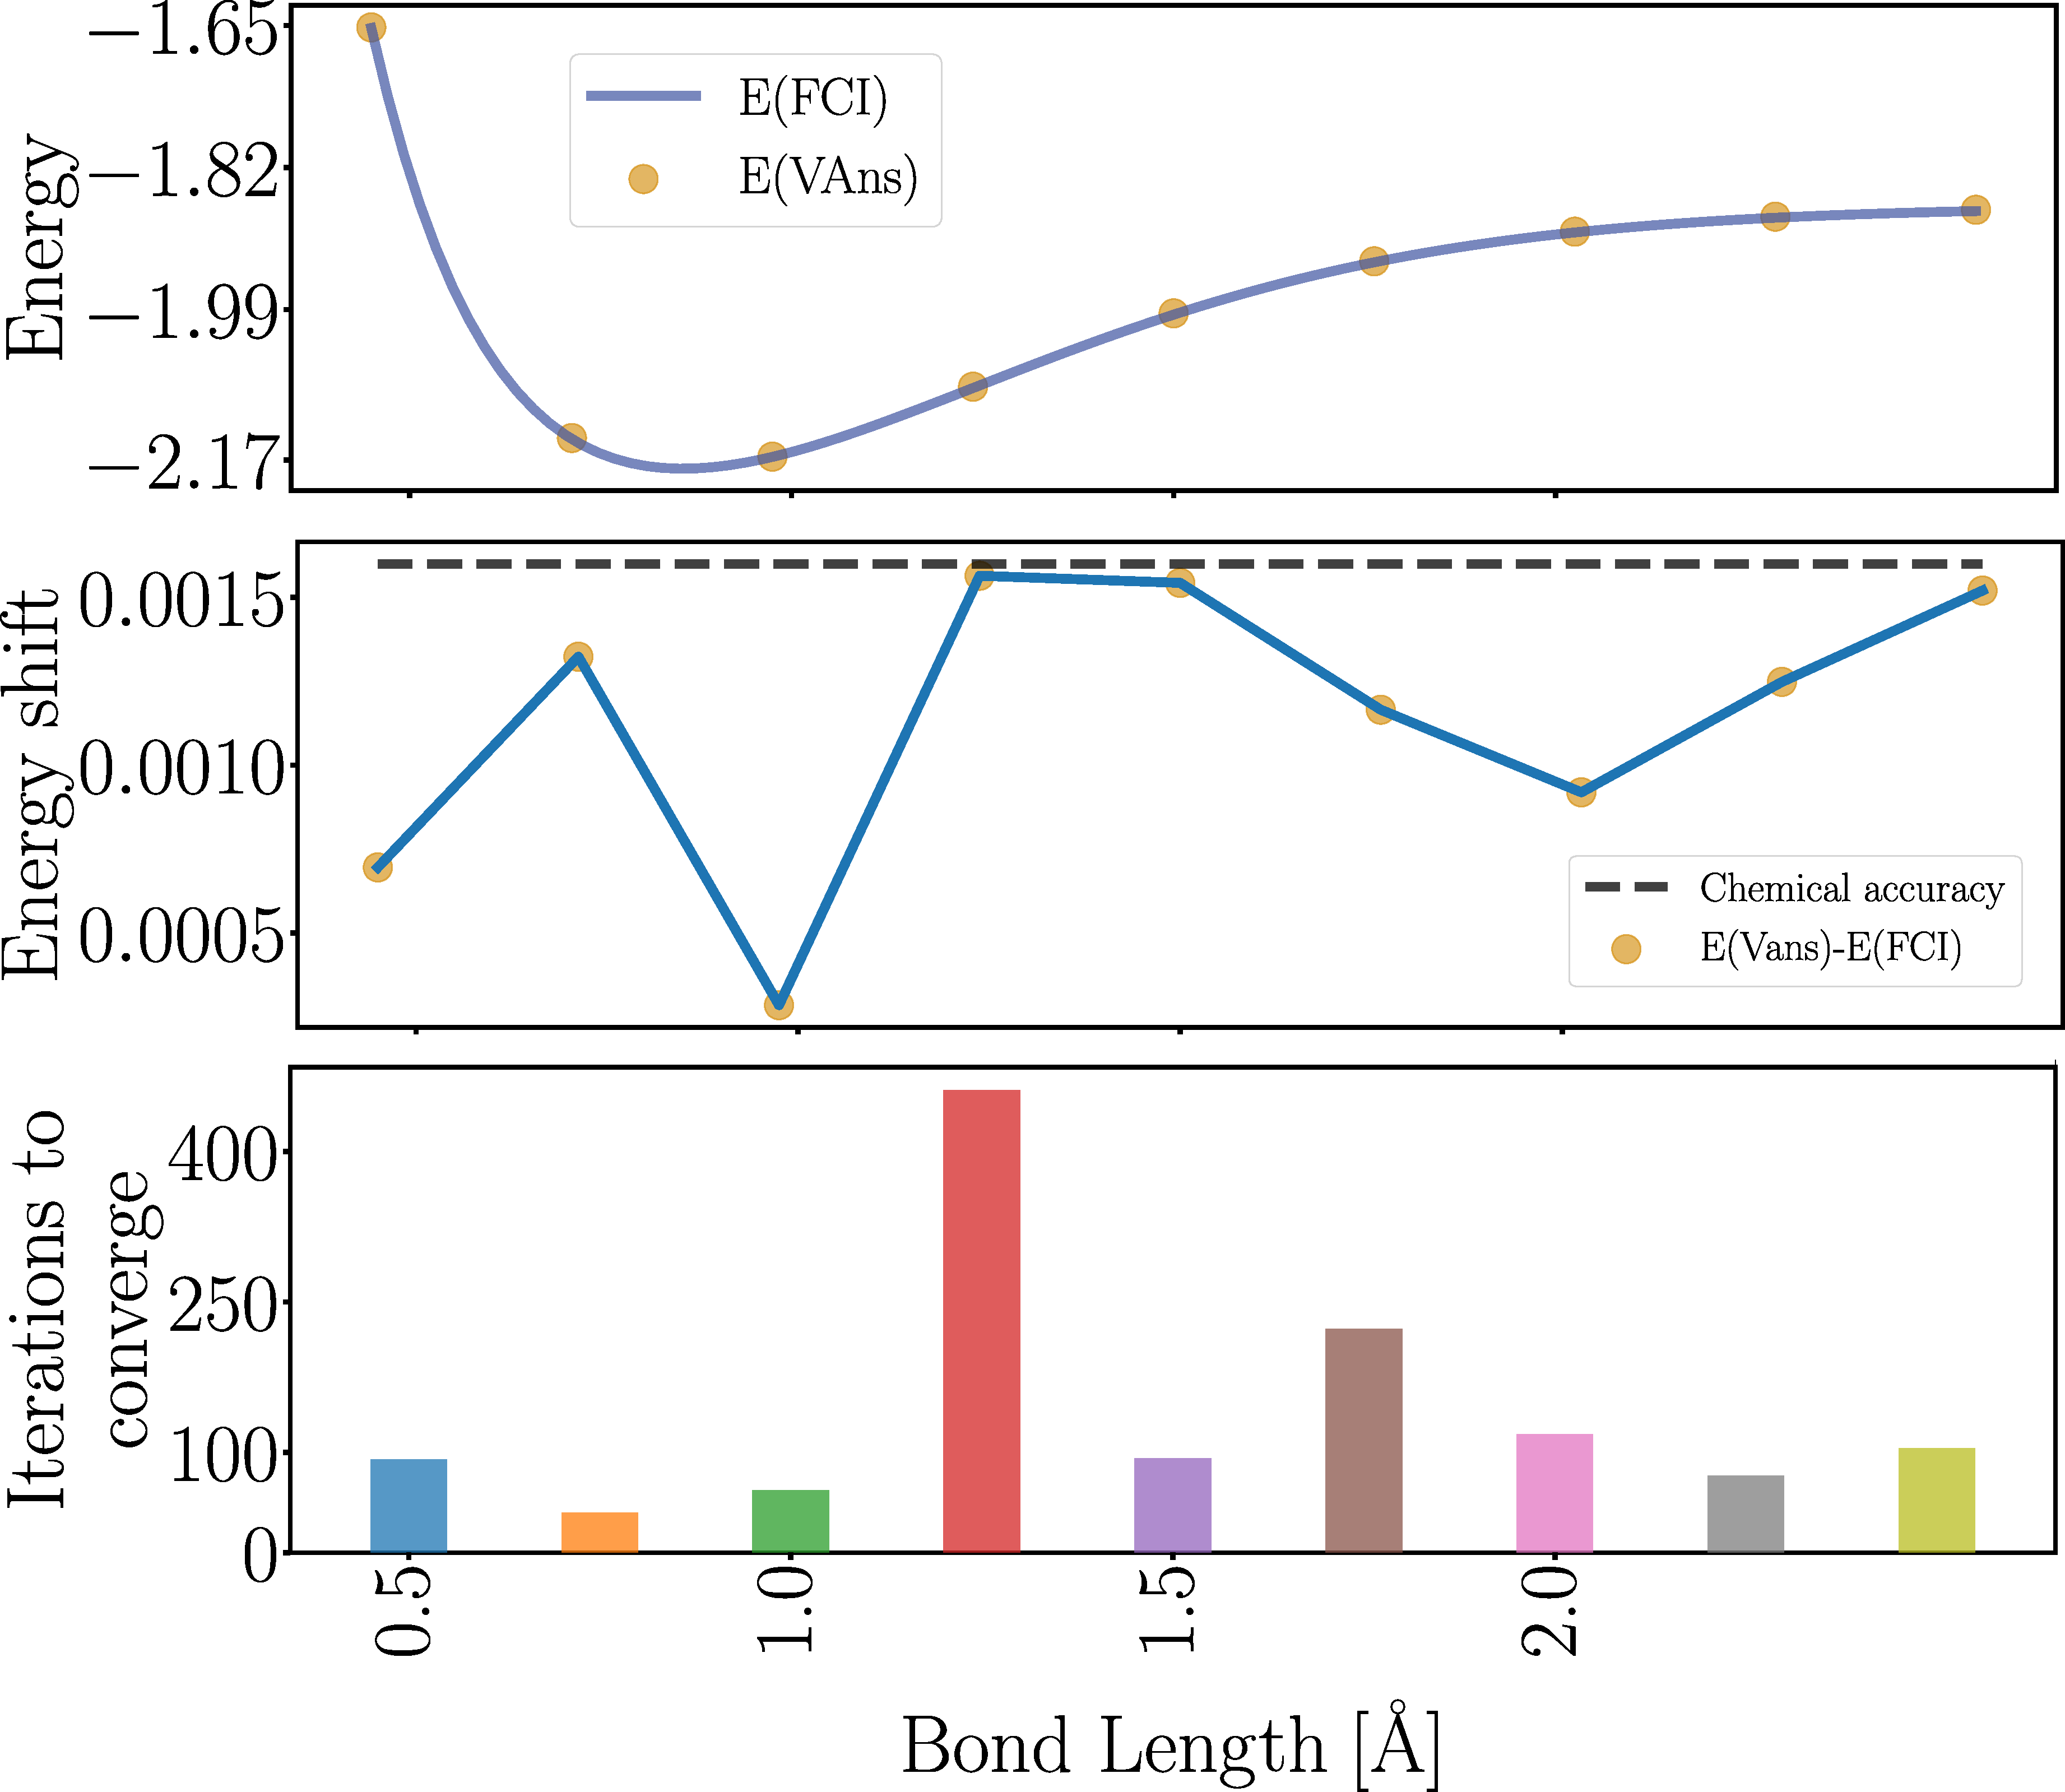
\includegraphics[width=1.\textwidth]{Figures/VANS/Fig12.pdf}
      \caption{}
      \label{fig:h24}
  \end{subfigure}
\caption{We show results of using VAns to obtain the ground state of a Hydrogen (H4) molecule, at different bond lengths (for the H4 molecule, this means the distance between the equally-separated atoms, which are disposed in a lineal array). Here we use VAns in the VQE algorithm for the molecular Hamiltonian obtained after a Jordan-Wigner transformation, leading to a 4(8)-qubit circuit in left(right) panels. Top: Solid lines correspond to ground state energy as computed by the Full Configuration Interaction (FCI) method, whereas points correspond to energies obtained using VAns. Middle: Differences between exact and VAns ground state energies are shown. Dashed line corresponds to chemical accuracy, which stands for the ultimate accuracy experimentally reachable in such systems. Bottom: Number of iterations required by VAns until convergence are shown.}
\label{fig:H4}
\end{figure}

\clearpage

\subsection{Quantum Autoencoder}
We will now focus on the quantum autoencoder. This is a paradigmatic quantum-machine learning application which was first introduced in~\cite{romero2017quantum}, where the quantum information stored in a multipartite quantum state is aimed to be compressed in terms of qubits' number. %This means that while $N$ qubits are required in order to store the initial state, a succesful training of the quantum autoencoder will lead to an approximate version of such state, requiring only $K<N$ qubits (and $N-K$ ancillas).

In the following, we will first introduce the quantum-autoencoder and then study how VANs can be applied to train it. In particular we will show results when using VAns to train the autoencoder to compress the ground-states of the Hydrogen molecule, from $4$ qubits to $2$.

\begin{figure}[t!]
\centering

\includegraphics[width=1.\textwidth]{Figures/VANS/Fig10.pdf}
\caption{Schematic diagram of the quantum autoencoder implementation. We first employ VAns to learn the circuits that prepare the ground states $\{\ket{\psi_i}\}_{i=1}^M$ of the $H_2$ molecule for different bond lengths. These ground states are then used to create a training set and test set for the quantum autoencoder implementation. The goal of the autoencoder is to train an encoding parametrized quantum circuit $V(\kvec, \thv)$ to compress each $\ket{\psi_i}$ into a subsystem of two qubits so that one can recover $\ket{\psi_i}$ from the reduced states, and we quantify this using the cost in Eq.~\ref{eq:costautoencoderglobal}.}
\label{fig:AE}
\end{figure}

We consider a bipartite quantum system $AB$ of $n_A$ and $n_B$ qubits, respectively. Let $\{p_i,\ket{\psi_i}\}$ be a training set of pure states on $AB$. The goal of the quantum autoencoder is to train an encoding parametrized quantum circuit $V(\kvec, \thv)$ to compress the states in the training set onto subsystem $A$, so that we can discard the qubits in subsystem $B$ without losing much information. This can be quantified by introducing an ancillary system $B'$, and computing how close can the autoencoder transformation get to the initial training set. The performance of this task can be quantified by the average fidelity between the input and output states (as a shorthand, we will denote $V(\kvec, \thv)$ as $V_{AB}$, when acting on the system (AB)).
\begin{align}C_1(\thv) &= 1- \sum_i p_i \cF(\ket{\psi_i}, \rho_{i,out}),\\
\rho_{i,out}&= V^\dagger_{AB'} \text{Tr}_B\Big[ V_{AB} \Big( [\psi_{i,AB}] \otimes [0_{B'}] V_{AB}^\dagger  ] \Big) \Big] V_{AB'},
\end{align}
where we note that $\rho_{i,out}\in \mathcal{H}_{AB'}$ (for our purposes, $B'$ is just a copy of $B$, and they have the same dimension), and the autoencoder is represented by the unitary $V$ we aim to train. Moreover, we have used the notation $[\psi] = \proj{\psi}$, and denoted the fidelity between to states by $\cF$.

\begin{figure}[t!]
\centering
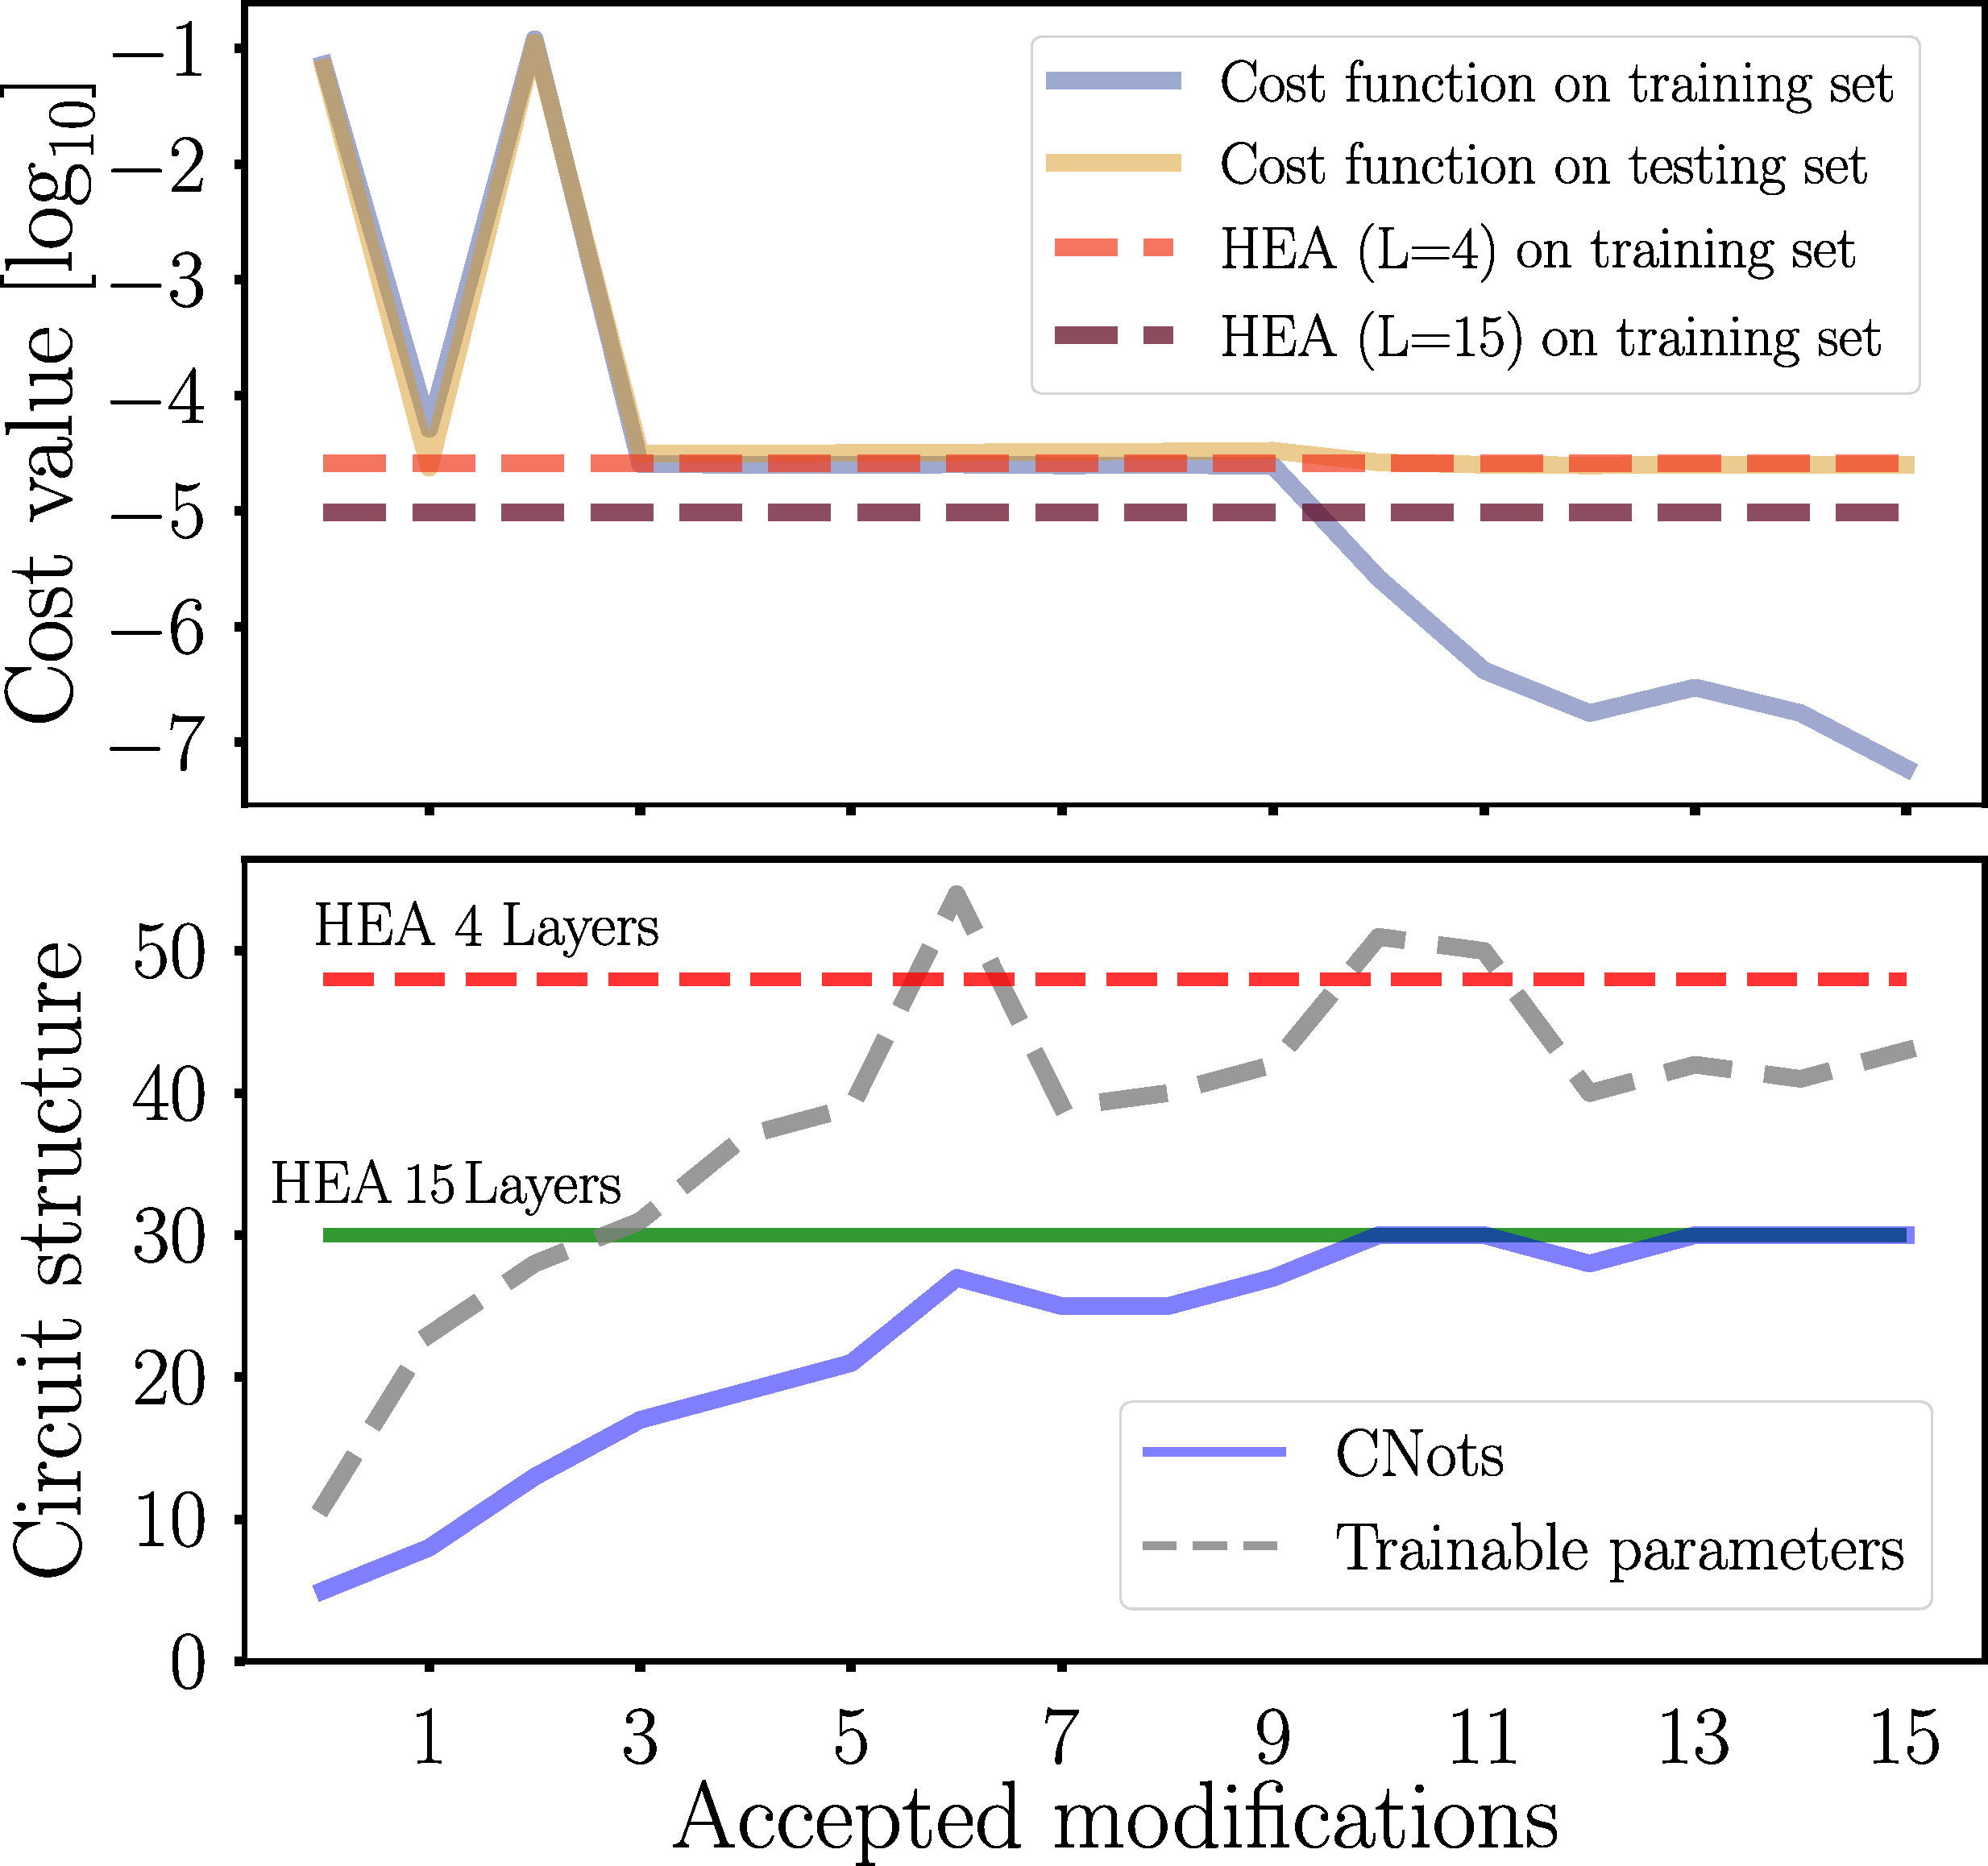
\includegraphics[width=.8\textwidth]{Figures/VANS/Fig11.pdf}
\caption{ {\small Results of using VAns to train a quantum autoencoder. Here we use VAns to train an encoding parametrized quantum circuit by minimizing Eq.~\eqref{eq:costautoencoderglobal} on a training set comprised of six ground states of the hydrogen molecule. We here also show the lowest cost function obtained for a $L$-HEA of $L=4$ and $L=15$ layers. Top panel: the cost function evaluated at both versus accepted VAns circuit modifications. In addition, we also show results of evaluating the cost on the testing set. Bottom panel: number of CNOTs, and number of trainable parameters versus the number of modifications of the ansatz accepted in the VAns algorithm. Here we additionally  show the number of CNOTs (solid line) and parameters (dashed line) in the HEA ansatzes considered. We remark that for 15-HEA has $180$ parameters, and hence the curve is not shown as it would be off the scale.}
}
\label{fig:AE_results}
\end{figure}
%

Thus, the quantum autoencoder consists on the following steps:
\begin{itemize}
\item Encode the quantum state $\ket{\psi_{i,AB}}$ to obtain $[\psi'_{AB}] = V_{AB} \Big( [\psi_{i,AB}]\Big) V_{AB}^\dagger$.
\item Discard the $B$ system by tracing over it.
\item Construct a new version of the global system $AB'$, by introducing a reference state $[0_{B'}]$ in $B'$. This results in an state $\text{Tr}_B [\psi'_{i,AB}] \otimes [0_B']$; we can think on the previous step and this one as reseting the state of sub-system $B$ to $[0_B']$.
\item Decode the quantum state to obtain an approximate version of $\ket{\psi_i}$ by revering the unitary transformation (\textit{e.g.} by applying $V^\dagger$).
\end{itemize}

Thus, $V$ is aimed to decouple subsystem $A$ from subsystem $B$, so that the resulting state is completely compressed into subsystem $A$ if the qubits in $B$ are found in the fixed target state $[0_{B}]$. In turn, assuming that $V\ket{\psi_{i,AB}} = \ket{\phi_{i,A}}\ket{0_B}$, then it follows that $\rho_{i,out} = [\psi_{i,AB'}]$, which lead to an average fidelity of $1$.

As shown in~\cite{romero2017quantum}, optimizing the average fidelity between the input and output states is equivalent to impose that the reduced state of system $B$, known as \textit{trash state} \textit{e.g.} $\text{Tr}_A [\psi'_{i,AB}]$ after encoding, matches the reference state $[0_{B'}]$. \footnote{To compute this, we need to introduce a swap operation between $B$ and $B'$, which we omitted in the discussion.}. Inspired by this, and the fact that computing the fidelities (for instance, via the SWAP) test requires a considerably comlex circuit, whose compilation would lead to potentially many gates in the NISQ-context, Ref.~\cite{romero2017quantum} considers an alternative cost-function of the form
\begin{equation}\label{eq:costautoencoderglobal}
    C(\kvec,\thv)=1-\sum_ip_i\tr{\left(\dya{0}_B\otimes \id_A\right)V\dya{\psi_i}V^\dagger}\,
\end{equation}
where $\id_A$ is the identity on subsystem $A$. Here we see that if the reduced state in $B$ is $\ket{0}_B$ for all the states in the training set, then the cost is zero.

As shown in Fig.~\ref{fig:AE}, we employ the ground states $\ket{\psi_i}$ of the $H_2$ molecule (for $M$ different bond lengths) to create a training set of six states and a test set of ten states. Here, the circuits obtained through VAns in the previous section serve as (fixed) state-preparation circuits for the $H_2$-molecule ground-states. We then use VAns to learn an encoding circuit $V(\kvec, \thv)$ which can compress the states $\ket{\psi_i}$ into a subsystem of two qubits.

Fig.~\ref{fig:AE_results} presents results obtained by minimizing the cost in Eq.~\ref{eq:costautoencoderglobal}, for a single run of the VAns algorithm. As seen, within $15$ accepted architecture modifications, VAns can decrease the training cost function down to $10^{-7}$, by departing from a separable product ansatz (see Fig.~\ref{fig:FANSATZ}). We here additionally show results obtained by training the Hardware Efficient Ansatz of Fig.~\ref{fig:FANSATZ}(b) with $4$ and $15$ layers
(as they have a comparable number of trainable parameters and CNOTs, respectively, compared to those obtained with VAns). In all cases, VAns achieves the best performance. In particular, it is worth noting that VAns has much fewer parameters
($\sim 45$ versus 180) than the 15-layer HEA, while also achieving a cost value that is lower by two orders of magnitude. Hence, VAns obtains better performance with fewer quantum resources.

To end this Section showcasing VAns in ideal scenarios, we will now discuss the case of unitary compilation.

\subsection{Unitary compilation} \label{sec:unitary_compilation}
Unitary compilation is a task in which a target unitary is decomposed into a sequence of quantum gates that can be implemented on a given quantum computer. As discussed in Sec.~\ref{sec:1_nisq}, current quantum computers are limited by the depth of quantum circuits that can be executed on them, which makes the compilation task very important in the near term. Indeed, we would like to decompose a given unitary using as few gates as possible to maximally reduce the effect of noise. %In this section we show that VAns is capable of finding very short decompositions as compared with other techniques.

We will illustrate our approach by compiling Quantum Fourier Transform (QFT) on systems up to $n=10$ qubits. Apart from VAns, we also compile the QFT unitary using standard HEA and compare the performance of both methods.

The cost function for unitary compilation is defined as follows. First, a training set is selected
\begin{equation} \label{eq:UC_training_set}
	\{ \big(
	\ket{\psi_j} , U_\mathrm{QFT}^{(n)} \ket{\psi_j}
	\big) \}_{j=1}^M \ ,
\end{equation}
where $U_\mathrm{QFT}^{(n)}$ is a target QFT unitary on $n$ qubits and $\ket{\psi_j}$ are $M$, randomly selected input states. We assume that the states $\ket{\psi_j}$ are pairwise orthogonal to avoid potential optimization problems caused by similarities in the training set. The cost function takes the form
\begin{equation} \label{eq:UC_cost}
	C(\kvec,\thv) = \sum_{j=1}^N
	|| U_\mathrm{QFT}^{(n)}\ket{\psi_j} -
	V(\kvec,\thv) \ket{\psi_j} ||^2 \ .
\end{equation}
Note that the cost function introduced in Eq.~\eqref{eq:UC_cost} becomes equivalent to a more standard one, $C'(\kvec,\thv) = || U_\mathrm{QFT}^{(n)} - V(\kvec,\thv)||^2$, when $M=2^n$. While $C(\kvec,\thv)$ measures the distance between the exact output of QFT and the one returned by $V(\kvec,\thv)$ only on selected input states, $C'(\kvec,\thv)$ measures the discrepancy between full unitaries $U_\mathrm{QFT}^{(n)}$ and $V(\kvec,\thv)$.
%
It has recently been shown~\cite{caro2021generalization} that $M \ll 2^n$ is sufficient to accurately decompose $U_\mathrm{QFT}^{(n)}$. More precisely, a constant number of training states $M$ (independent of $n$) can be used to ensure small value of $C'(\kvec,\thv)$, while minimizing the cost function in Eq.~\ref{eq:UC_cost}.
This observation provides an exponential speedup in evaluating the cost function for unitary compilation. Indeed, the cost of evaluating $C(\kvec,\thv)$ in Eq.~\eqref{eq:UC_cost} is $M \cdot 2^n$ (assuming the circuit $V(\kvec,\thv)$ consists of few body gates and the states $U_\mathrm{QFT}^{(n)} \ket{\psi_j} $ are given in computational basis), while the cost of computing $C'(\kvec,\thv)$ is $4^n$.
%
The number of training states $M$ which lead to small value of $C'(\kvec,\thv)$ depends on the number of independent variational parameters in $V(\kvec,\thv)$. Suboptimal decompositions $V(\kvec,\thv)$ (in terms of number of parametrized gates) will require larger $M$ to achieve good compilation accuracy. We have used $M = 15$ for $n=10$ qubit compilation with VAns, and a much larger training set in an approach that uses HEA; the increase in $M$ is necessary since the latter approach needed a much deeper circuit, as discussed below.
%
We have used most general two-qubit gates as the building block in VAns and to construct HEA. This is a slight generalization to the \texttt{Insertion} and \texttt{Simplification} steps in the VAns algorithm discussed above. % The optimization over $\thv$ was performed with qFactor~\cite{qFactor}.
General two-qubit gates can be decomposed in terms of CNOTs and one-qubit rotations using standard methods.

The method based on HEA requires very deep circuits (at $n=10$). They consists of so many gates that the regular optimization has very small success probability. We therefore modify the method based on HEA and utilize the recursive structure of $U_\mathrm{QFT}^{(n)}$. In the modified approach, we use HEA to compile $U_\mathrm{QFT}^{(n-1)}$ and then use it to create an ansatz for $U_\mathrm{QFT}^{(n)}$. The ansatz for larger system size additionally consists of several layers of HEA. We apply the above growth technique starting from $n=3$ to eventually build the ansatz for $n=10$. We stress that VAns does not require such simplification and is capable of finding the decomposition  with high success probability directly at $n=10$ while initialized randomly.

\begin{figure}[t!]
\centering
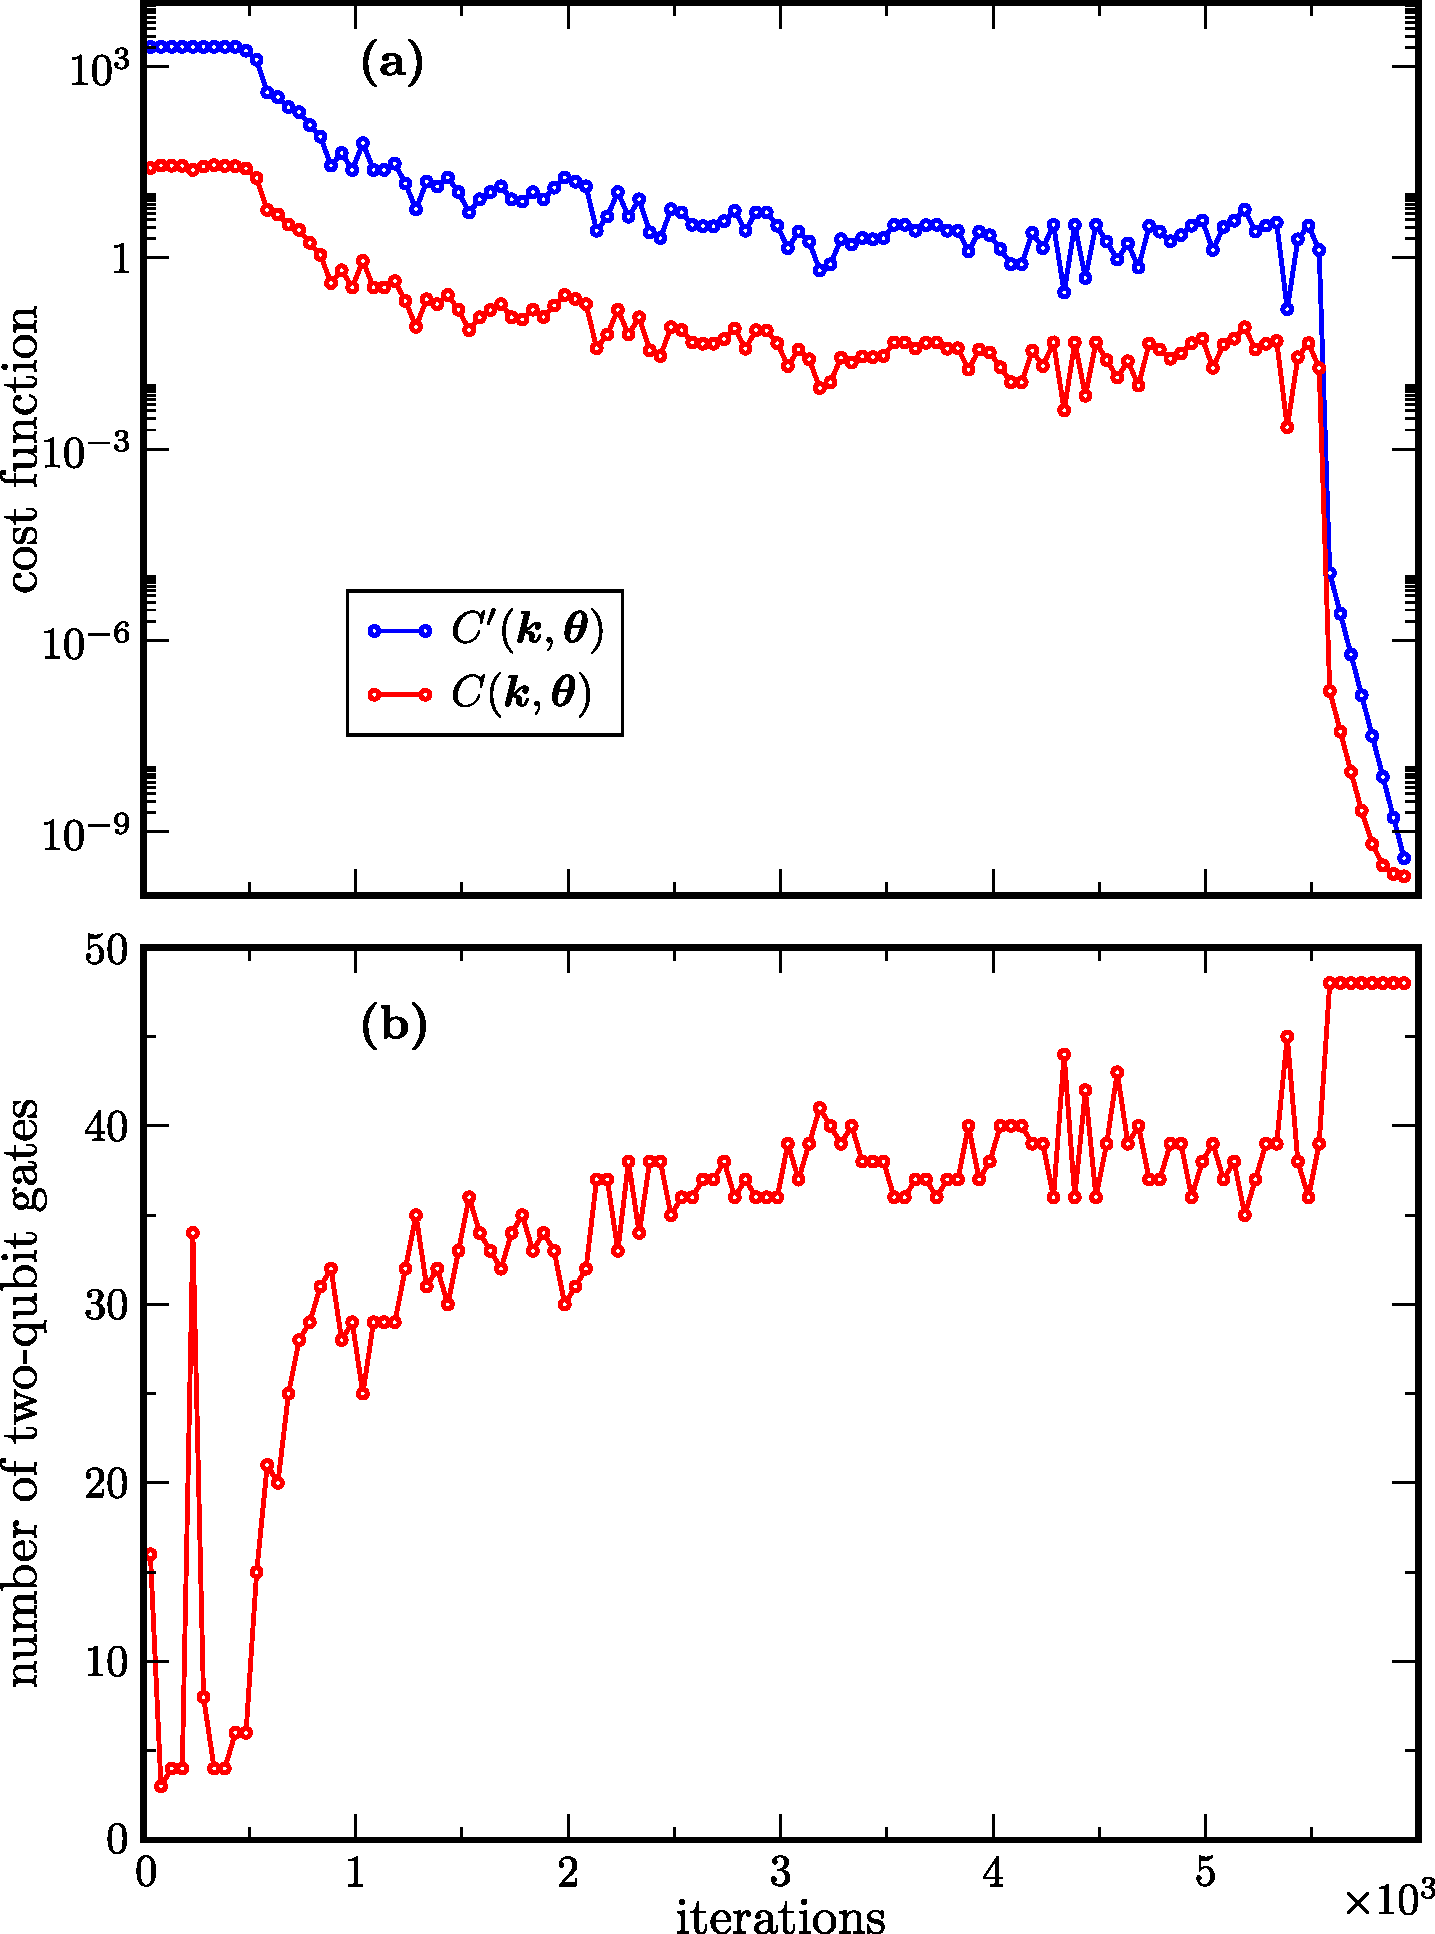
\includegraphics[width=.75\textwidth]{Figures/VANS/unitary_compilation.pdf}
\caption{Results of using VAns for unitary compilation. Here we use VAns to find a decomposition of QFT unitary defined on $n=10$ qubits, by minimizing a cost function $C(\kvec,\thv)$ (red line in panel \textit{(a)} defined in Eq.~\eqref{eq:UC_cost}. The cost evaluates a difference between exact output of QFT and the one returned by a current circuit, on a small number of input states only ($M=15$). The blue line shows corresponding difference between full unitaries, $C'(\kvec,\thv) = || U_\mathrm{QFT}^{(n)} - V(\kvec,\thv)||^2$. We observe a high correlation between those two cost functions. Panel \textit{(b)} shows how VAns modifies the number of two-qubit gates as it approaches the minimum of $C(\kvec,\thv)$.
The minimum is found with 48 gates, which is $\sim 4.5$ times less than the decomposition found with HEA (not shown).
}
\label{fig:unitary_compilation_results}
\end{figure}
\afterpage{\clearpage}

Figure~\ref{fig:unitary_compilation_results} shows VAns results for $n=10$ qubit QFT compilation. Panel (a) depicts how the value of the cost function $C(\kvec,\thv)$ is minimized over the iterations. We also show the corresponding value of $C'(\kvec,\thv) = || U_\mathrm{QFT}^{(n)} - V(\kvec,\thv)||^2$.
We observe strong correlation between both cost functions. $C'(\kvec,\thv)$ is eventually minimized below $10^{-9}$ at the end of the optimization. Panel \textit{(b)} shows how the number of two-qubit gates evolves as VAns optimization is performed. Excluding the initial \textit{warm-up} period, during which the cost function has very large (close to maximal possible) value, the number of two-qubit gates %def 2-qubit gate, are the general 2-qubit gates? in terms of CNOTs? 12 each right?
is steadily grown reaching 48 at the end of the optimization.
That number is only slightly larger than the number of two-qubit gates (45) used in the textbook-QFT circuit for $n=10$.

The approach based on HEA requires 219 general two-qubit gates to decompose $n=10$ QFT, which is over 4 times more than the best circuit found by VAns. The HEA approach uses recursive structure of QFT to find accurate decomposition, while VAns does not rely on that property and finds a solution in fewer number of iterations. Finally, VAns takes advantage of the generalization bound \cite{caro2021generalization}, finding solution with near optimal number of variational parameters in $V(\kvec,\thv)$; the training set size $M$ required for small generalization error is small resulting in fast cost function evaluations.
\afterpage{\clearpage}
